%%%%%%%%%%%%%%%%%%%%%%%%%%%%%%%%%%%%%%%%%%%%%%%%%%%%%%%%%%
%
% Vzor pro sazbu kvalifikační práce
%
% Západočeská univerzita v Plzni
% Fakulta aplikovaných věd
% Katedra informatiky a výpočetní techniky
%
% Petr Lobaz, lobaz@kiv.zcu.cz, 2016/03/14
%
%%%%%%%%%%%%%%%%%%%%%%%%%%%%%%%%%%%%%%%%%%%%%%%%%%%%%%%%%%

% Možné jazyky práce: czech, english
% Možné typy práce: BP (bakalářská), DP (diplomová)
\documentclass[czech,BP]{thesiskiv}

% Definujte údaje pro vstupní strany
%
% Jméno a příjmení; kvůli textu prohlášení určete, 
% zda jde o mužské, nebo ženské jméno.
\author{Petr Kozler}
\declarationmale

%alternativa: 
%\declarationfemale

% Název práce
\title{Vytvoření knihoven s~definovaným rozhraním v~jazycích C, C++, C\# a FreePascal}

% 
% Texty abstraktů (anglicky, česky)
%
\abstracttexten{This work examines the possibilities of transfer the source code written in the Java programming language to the C, C++, C\# and Pascal programming language. The first part is the research of the availability of libraries with functionality similar to the commonly used Java libraries in those other languages. The next part is implementation of libraries providing Java-like interfaces in other listed languages using the available libraries of these languages, as well as design and implementation of application which allows to search in, view and manipulate their source code. The work should provide a convenient way to translate the code using common Java libraries to the listed languages while keeping its functionality and outline the ways to convert another libraries or imitate the behavior of them in another languages.}

\abstracttextcz{Tato práce se zabývá převodem zdrojových kódů psaných v~programovacím jazyku Java do programovacích jazyků C, C++, C\# a Pascal. V~první části zkoumá dostupnost knihoven s~funkcionalitou podobnou základním knihovnám jazyka Java v~ostatních uvedených jazycích. Další částí práce je implementace knihoven poskytujících rozhraní v~duchu jazyka Java v~ostatních uvedených jazycích a využívajících knihovny těchto jazyků a dále návrh a implementace aplikace umožňující vytvořené zdrojové kódy vyhledávat, zobrazovat a dále s~nimi manipulovat. Práce by měla umožnit snadný překlad kódu využívajícího základní knihovny jazyka Java do uvedených jazyků se zachováním jeho funkcionality a nastínit způsoby, jakými lze převádět další knihovny do uvedených jazyků nebo napodobit jejich chování v~dalších jazycích.}

% Na titulní stranu a do textu prohlášení se automaticky vkládá 
% aktuální rok, resp. datum. Můžete je změnit:
%\titlepageyear{2016}
%\declarationdate{1. března 2016}

% Ve zvláštních případech je možné ovlivnit i ostatní texty:
%
%\university{Západočeská univerzita v Plzni}
%\faculty{Fakulta aplikovaných věd}
%\department{Katedra informatiky a výpočetní techniky}
%\subject{Bakalářská práce}
%\titlepagetown{Plzeň}
%\declarationtown{Plzni}

%%%%%%%%%%%%%%%%%%%%%%%%%%%%%%%%%%%%%%%%%%%%%%%%%%%%%%%%%%
%
% DODATEČNÉ BALÍČKY PRO SAZBU
% Jejich užívání či neužívání záleží na libovůli autora 
% práce
%
%%%%%%%%%%%%%%%%%%%%%%%%%%%%%%%%%%%%%%%%%%%%%%%%%%%%%%%%%%

% Zařadit literaturu do obsahu
\usepackage[nottoc,notlot,notlof]{tocbibind}

% Umožňuje vkládání obrázků
\usepackage[pdftex]{graphicx}

% Odkazy v PDF jsou aktivní; navíc se automaticky vkládá
% balíček 'url', který umožňuje např. dělení slov
% uvnitř URL
\usepackage[pdftex]{hyperref}
\hypersetup{colorlinks=true,
  unicode=true,
  linkcolor=black,
  citecolor=black,
  urlcolor=black,
  bookmarksopen=true}

% Při používání citačního stylu csplainnatkiv
% (odvozen z csplainnat, http://repo.or.cz/w/csplainnat.git)
% lze snadno modifikovat vzhled citací v textu
\usepackage[numbers,sort&compress]{natbib}

%%%%%%%%%%%%%%%%%%%%%%%%%%%%%%%%%%%%%%%%%%%%%%%%%%%%%%%%%%
%
% VLASTNÍ TEXT PRÁCE
%
%%%%%%%%%%%%%%%%%%%%%%%%%%%%%%%%%%%%%%%%%%%%%%%%%%%%%%%%%%
\begin{document}
%
\maketitle
\tableofcontents

\chapter{Úvod}
Cílem této práce je usnadnit překlad programového kódu z~programovacího jazyka \textit{Java} do jiných programovacích jazyků. Konkrétně se bude jednat o~jazyky \textit{C}, \textit{C++}, \textit{C\#} a \textit{Pascal} v~dialektu překladače Free Pascal. Práce bude sestávat ze čtyř hlavních kroků.\par
Prvním krokem bude seznámení se s~dostupností funkcionality různých běžně používaných metod a tříd z~jazyka Java v~ostatních výše uvedených jazycích a průzkum toho, jak v~těchto jazycích fungují. Předmětem zkoumání bude především paradigma jednotlivých jazyků, dále typový systém, funkce, popř. metody pro matematické výpočty, kontejnery (zejména statická a dynamicky zvětšovaná pole a spojové seznamy), řetězce, funkce nebo metody pro práci s~kontejnery (např. řazení a vyhledávání prvků) a funkce, popř. třídy pro vstupní a výstupní operace. Účelem zkoumání bude nalezení nejsnadnějších (s~ohledem na efektivitu a přehlednost zdrojového kódu) dostupných způsobů, jak v~daných jazycích vytvořit konstrukci funkčně odpovídající danému řešení z~jazyka Java.\par
Druhým krokem bude vytvořit v~těchto jazycích knihovny s~rozhraním ve stylu jazyka Java, obalující tyto konstrukce. To bude realizováno způsobem, který umožní jejich použití s~minimálním počtem úprav zdrojového kódu z~jazyka Java, který bude tyto konstrukce využívat, se současným úplným zachováním požadované funkčnosti.\par
Třetím krokem bude vytvoření aplikace v~jazyce Java, která bude sloužit ke správě vytvořených knihoven. Aplikace bude disponovat grafickým uživatelským rozhraním a bude umožňovat jedoduché vyhledávání, zobrazení, přidávání, úpravy a odstraňování jednotlivých knihoven i programovacích jazyků. Data aplikace představující zdrojové kódy knihoven budou ukládána do souborů ve formátu XML. Na chybné vstupy bude aplikace reagovat vhodným hlášením, z~něhož bude patrná příčna problému.\par
Posledním krokem bude otestování celého programového vybavení. Základním prvkem testování budou jednotkové testy, které budou mít za úkol prověřovat, zda se výstupy jednotlivých funkcí nebo metod implementovaných v~jazycích C, C++, C\# a Pascal shodují s~výstupy odpovídajících metod v~jazyce Java, a zda chování aplikace pro správu zdrojového kódu odpovídá očekáváním.

\chapter{Analýza metod a funkcí programovacích jazyků}
V~této kapitole budou popsány charakteristiky jednotlivých jazyků a různé základní funkce a metody, které tyto jazyky poskytují. 

\section{Obecná charakteristika}
Základní rozdíly mezi popisovanými jazyky jsou mj. ve způsobu zpracování zdrojového kódu, programovacím paradigmatu, správě paměti a syntaxi.

\subsection{Java}
Java je názvem technologie, jejíž součástí je kromě stejnojmenného vysokoúrovňového (poskytujícího vysokou úroveň abstrakce) \textit{objektově orientovaného} programovacího jazyka i softwarová platforma pro běh programů v~tomto jazyce vytvořených. Z~hlediska způsobu překladu a spuštění zdrojového kódu se nejedná o~čistě kompilovaný ani interpretovaný jazyk, ale o~hybridní jazyk. Zpracování programového kódu probíhá následovně \cite{java-book, java-guide-vm, java-guide-javac, java-guide-java}:
\begin{enumerate}
\item Nejprve je proveden překlad veškerého zdrojového kódu (ukládaného do textových souborů, které mají příponu \texttt{.java}) s~pomocí kompilátoru \texttt{javac} do tzv. mezijazyka zvaného \textit{bajtkód}, angl. bytecode (ukládaného v~souborech s~příponou \texttt{.class}). Bytecode je jednodušší formou kódu -- jedná se o~strojový kód \textit{virtuálního stroje} zvaného Java Virtual Machine (dále jen JVM). 
\item Virtuální stroj JVM následně interpretuje (po spuštění nástrojem \texttt{java}) kód \texttt{.class} souboru do nativního kódu cílového procesoru. 
\end{enumerate}
Stejný kód je tedy možné spustit na různých platformách (resp. na platformách, pro které je JVM k~dispozici) \cite{java-book}.\par
Jednou ze základních vlastností jazyka Java je \textit{automatická správa paměti}. Ta umožňuje vytváření objektů bez nutnosti jejich explicitního odstranění za účelem uvolnění paměti ve chvíli, kdy již nejsou potřeba. Objekty, které se nadále nepoužívají (nevedou na ně již žádné odkazy), jsou běhovým prostředím odstraňovány automaticky. Proces automatického likvidování objektů se nazývá garbage collection \cite{java-book, java-guide-vm}.
Syntax jazyka je zjednodušenou a mírně upravenou podobou syntaxe jazyků C a C++. Objektový model jazyka je založený na třídách a jazyk podporuje genericitu. S~výjimkou základních datových typů jsou všechny proměnné objektem (instancí třídy). Kořenem stromové hierarchie dědičnosti tříd je třída \texttt{java.lang.Object} – každá třída je tedy potomkem třídy \texttt{java.lang.Object}. Třídy, popř. další konstrukce (rozhraní, výčtové typy) mohou být seskupovány do jmenných prostorů, tzv. balíků (packages) \cite{java-book, java-guide-object}.\par

\subsection{C}
C je nízkoúrovňový, strukturovaný, na funkcích založený jazyk. Pojem nízkoúrovňový znamená, že jazyk přímo pracuje jen se základními datovými typy (znaky, čísla), poskytuje tedy nižší úroveň abstrakce než objektově orientované jazyky jako je např. jazyk Java. Výhodou tohoto přístupu je relativní jednoduchost vytvoření kompilátoru pro konkrétní platformu a efektivita kódu \cite{c-book, c-guide}.\par
Jak již bylo nastíněno, na rozdíl od jazyka Java se jedná o~jazyk čistě kompilovaný. Kompilace zdrojového kódu jazyka C sestává z~několika fází \cite{c-book, c-guide}:
\begin{enumerate}
\item \textit{Předzpracování} -- zpracování kódu tzv. preprocesorem, které spočívá v~úpravě kódu do podoby pro snadnější překlad. Součástí této úpravy je např. odstranění komentářů, rozvoj maker, vložení tzv. hlavičkových souborů (soubory s~příponu \texttt{.h}, obvykle obsahující např. prototypy funkcí, deklarace globálních proměnných nebo definice konstant a globálních typů a obvykle neobsahující výkonný kód) atd.
\item \textit{Překlad} -- program vykonávající tuto úlohu se nazývá kompilátor neboli překladač (angl. compiler). Jedná se o~hlavní část zpracování zdrojového kódu. Textový soubor kódu upraveného preprocesorem je převeden do objektového neboli relativního kódu cílového počítače (výsledkem práce kompilátoru je soubor \texttt{.obj}). Objektový kód představuje téměř hotový spustitelný soubor, pouze adresy proměnných a funkcí jsou zatím zapsány relativně (nejsou zatím známé, protože jsou např. uložené v~externí knihovně).
\item \textit{Sestavení} -- zpracování relativního kódu vytvořeného překladačem pomocí sestavovacího programu (angl. linker) zahrnuje přidělení absolutních adres a nalezení adres dosud neznámých identifikátorů (jako jsou volané funkce z~knihoven). Výstupem této fáze je již hotový program -- spustitelný soubor (v~OS Windows s~příponou \texttt{.exe}).
\end{enumerate}\par\noindent
Ze syntaxe tohoto jazyka je odvozena syntaxe všech ostatních jazyků uvedených v~této práci s~výjimkou jazyka Pascal. Na rozdíl od jazyků Java a C\# zde neexistuje mechanismus automatické správy paměti – alokace i dealokace paměti je úkolem programátora. K~tomuto účelu nicméně jazyk C poskytuje standardní knihovní funkce. Vzhledem k~nutnosti \textit{manuální správy paměti} obsahuje jazyk C na rozdíl od Javy nejen proměnné, obsahující přímo hodnoty, ale též proměnné nazývané jako ukazatele (angl. pointer) na hodnoty daných typů. Ukazatel je proměnná, jejíž hodnotou je adresa v~paměti a na této adrese je teprve uložena hodnota (kromě ukazatelů na proměnné existují též ukazatele na funkce). Právě s~pomocí ukazatelů jsou v~jazyce C realizovány konstrukce podobné složitějším typům jazyka Java, jako jsou řetězce a pole. Objekty jazyka Java lze částečně napodobit s~využitím konstrukcí jazyka C pro vytváření nehomogenních (složených z~různých datových typů) datových struktur \cite{c-book, c-guide}.

\subsection{C++}\label{sec:cpp-overview}
C++ je jazyk, který je nadstavbou jazyka C -- každý platný program v~jazyku C je tedy zároveň platným programem v~jazyku C++. Princip zpracování zdrojového kódu je stejný jako v~případě jazyka C (některé překladače fungují, nebo dříve fungovaly tak, že nejprve převedli zdrojový kód C++ na zdrojový kód C, který byl poté předán překladači jazyka C) \cite{cpp-book}.\par
Stejně jako jazyk C i jazyk C++ vyžaduje manuální správu paměti. Pro tento účel jsou nicméně k~dispozici nové jazykové prostředky, např. konstruktory a destruktory nebo reference na proměnné (jako alternativa k~ukazatelům). Kromě toho obsahuje jazyk C++ řadu dalších nových konstrukcí, jednou z~nejdůležitějších je třída. Rozdílem oproti C je tedy mj. podpora objektově orientovaného programování (vedle procedurálního přístupu z~jazyka C) a generického programování (prostřednictvím tzv. šablon). Jazyk C++ lze proto označit jako multiparadigmatický \cite{cpp-book, cpp-guide-classes}.\par
Mezi další nové konstrukce patří jmenné prostory (obdoba balíků v~jazyku Java), přetěžování funkcí i operátorů, standardní parametry, výše zmíněné šablony, vložené (angl. inline) funkce a další. Kromě nových konstrukcí přináší C++ oproti C také rozsáhlou sadu nových knihoven, přičemž je stále možné používat i knihovny z~jazyka C \cite{cpp-book}.\par

\subsection{C\#}
C\# je vysokoúrovňový, objektově orientovaný jazyk vycházející z~jazyků, jako je C++ a Microsoft Visual Basic a je zaměřený především na vývoj aplikací pro platformu .NET Framework \cite{cs-book, cs-guide-basic}.\par
Způsob zpracování programového kódu je postaven na podobných principech jako v~případě jazyka Java. Obdobou JVM je \textit{Common Language Runtime} a obdobou bytecode je \textit{Microsoft Intermediate Language}. Syntax je velmi podobná jazyku Java, navíc ale obsahuje konstrukce jako jsou například částečné třídy (třídy, jejichž definice je rozdělena do více zdrojových souborů), delegáty, přetěžování operátorů (nejen metod), předávání parametrů metod referencí, struktury (třídy, jejichž instance jsou vytvářené na zásobníku) nebo bezznaménkové číselné datové typy \cite{cs-book, cs-guide-clr, cs-guide-msil, cs-guide-jit, cs-guide-types}.\par

\subsection{Pascal}
Pascal je, stejně jako C a C++, kompilovaný jazyk, pro který je k~dispozici řada překladačů (každý z~nich definuje mírně odlišnou podobu jazyka, tzv. dialekt). Jedním z~nich je i volně šiřitelný překladač \textit{Free Pascal}, který je použit v~rámci této práce. Všechny poznámky týkající se Pascalu se tedy vztahují na dialekt překladače Free Pascal a nemusejí platit pro ostatní překladače \cite{pas-book}.\par
Vedle způsobu zpracování kódu je Pascal srovnatelný s~jazykem C++ také po stránce správy paměti a v~podporovaných programovacích paradigmatech -- je tedy podporováno jak strukturované programování založené na procedurách a funkcích (jako procedury jsou nazývány podprogramy bez návratové hodnoty), tak objektově orientované programování \cite{pas-book}.\par
Na první pohled odlišná je syntax jazyka, která je méně úsporná a je přizpůsobena pro výuku. Soubor zdrojového kódu programu se nazývá modul nebo jednotka (angl. unit), obvyklá přípona souboru je \texttt{.pas} a zdrojový kód má pevně danou strukturu. Jeho základem je blok, který se skládá z~hlavičky, deklarace a příkazové části. Deklarační část může obsahovat podprogramy, které mají stejnou strukturu \cite{pas-book, pas-guide-about}.\par

\section{Základní datové typy}
Všechny uvedené jazyky jsou typované -- při deklaraci proměnné je nutné uvést její datový typ. Každý z~těchto jazyků poskytuje množinu základních datových typů. Jejich seznam spolu s~uvedenými rozsahy hodnot je uveden níže.

\subsection{Java}
Jazyk Java je (stejně jako ostatní uvedené jazyky) \textit{staticky typovaný}, což znamená, že každou proměnnou je nutné před použitím deklarovat a kromě jména je nutné uvést její datový typ, který určuje množinu povolených hodnot a operací nad nimi. K~dispozici je 8 primitivních datových typů (typů předdefinovaných jazykem, jejichž název je klíčovým slovem jazyka), z~toho 4 celočíselné, 2 pro reálná čísla, 1 znakový a 1 pro logické hodnoty. Všechny číselné datové typy jsou znaménkové \cite{java-book, java-guide-types}.\par

Jednotlivé datové typy, jejich význam, velikost v~paměti a rozsahy hodnot popisuje tabulka \ref{table:java-types}. Pro uvedené typy jsou k~dispozici tzv. \textit{obalové třídy}, umožňující další operace (mj. slouží k~uchovávání hodnot primitivních datových typů jako objektů pro použití v~kolekcích); např. \texttt{java.lang.Integer} nebo \texttt{java.lang.Long}, které např. umožňují použití hodnot číselných datových typů jako bezznaménkových. Kromě těchto typů poskytuje jazyk Java speciální podporu pro řetězce reprezentované třídou \texttt{java.lang.String} (popsány v~kapitole \ref{sec:strings}) \cite{java-guide-types, java-guide-byte, java-guide-short, java-guide-integer, java-guide-long, java-guide-float, java-guide-double, java-guide-boolean, java-guide-character}.

\begin{table}\centering
\caption{Základní datové typy jazyka Java}
\begin{tabular}{| l | l | l |}
\hline
\textbf{Název} & \textbf{Význam} & \textbf{Rozsah} \\ \hline
\texttt{byte} & celé číslo & $-2^7$ .. $2^7-1$ \\ \hline
\texttt{short} & celé číslo & $-2^{15}$ .. $2^{15}-1$ \\ \hline
\texttt{int} & celé číslo & $-2^{31}$ .. $2^{31}-1$ \\ \hline
\texttt{long} & celé číslo & $-2^{63}$ .. $2^{63}-1$ \\ \hline
\texttt{float} & reálné číslo & dle IEEE 754 (jednoduchá přesnost) \\ \hline
\texttt{double} & reálné číslo & dle IEEE 754 (dvojitá přesnost) \\ \hline
\texttt{boolean} & logická hodnota & \texttt{true} nebo \texttt{false} \\ \hline
\texttt{char} & znak Unicode & \texttt{'\textbackslash u0000'} ($0$) .. \texttt{'\textbackslash uffff'} ($2^{16} - 1$) \\ \hline
\end{tabular}
\label{table:java-types}
\end{table}

\subsection{C}
Primitivní datové typy jazyka C zahrnují typy celočíselné a typy pro reálná čísla (vestavěný typ pro logické hodnoty jazyk C neobsahuje, místo něj lze logické hodnoty reprezentovat pomocí hodnot celočíselného typu). Velikosti a rozsahy jednotlivých datových typů závisí na cílové platformě. Garantovány jsou pouze minimální rozsahy a pořadí velikosti rozsahů pro jednotlivé datové typy (není však vyžadováno, aby jednotlivé datové typy měly rozsahy rozdílné velikosti). Definice celočíselných datových typů s~garantovanými rozsahy hodnot obsahuje soubor \texttt{stdint.h}, přičemž některé z~nich jsou volitelné a jejich podpora proto není zaručena na všech platformách \cite{c-guide, cpp-guide-stdint}.\par

Minimální rozsahy základních typů jsou uvedené v~tabulce \ref{table:c-types}. Typy jsou seřazeny vzestupně podle minimální velikosti. Kromě uvedených datových typů existuje ke každému celočíselnému typu bezznaménková varianta -- její název začíná řetězcem \texttt{unsigned}. Takový typ má stejnou velikost jako příslušný znaménkový typ a jeho rozsah je posunutý tak, že nejmenší hodnota je 0 (tedy pouze kladná čísla). Celočíselné datové typy \texttt{long long int} a \texttt{unsigned long long int} nejsou součástí standardu C89. Konstanty představující hraniční hodnoty datových typů pro reálná čísla jsou uloženy v~hlavičkovém souboru \texttt{float.h} a platí pro ně, že typ \texttt{float} má nejmenší rozsah a zbylé dva typy mají rozsah minimálně tak velký, ale obvykle větší, než \texttt{float}. Konstanty plnící stejný účel pro celočíselné typy definuje soubor \texttt{limits.h} \cite{c-guide}.

\begin{table}\centering
\caption{Některé základní datové typy jazyka C}
\begin{tabular}{| l | l | l |}
\hline
\textbf{Název} & \textbf{Význam} & \textbf{Rozsah} \\ \hline
\texttt{char} & celé číslo & $-2^7$ .. $2^7-1$ \\ \hline
\texttt{short int} & celé číslo & $-2^{15}$ .. $2^{15}-1$ \\ \hline
\texttt{int} & celé číslo & $-2^{31}$ .. $2^{31}-1$ \\ \hline
\texttt{long int} & celé číslo & $-2^{31}$ .. $2^{31}-1$ \\ \hline
\texttt{long long int} & celé číslo & $-2^{63}$ .. $2^{63}-1$ \\ \hline
\texttt{float} & reálné číslo & \texttt{FLT\_MIN} .. \texttt{FLT\_MAX} \\ \hline
\texttt{double} & reálné číslo & \texttt{DBL\_MIN} .. \texttt{DBL\_MAX} \\ \hline
\texttt{long double} & reálné číslo & \texttt{LDBL\_MIN} .. \texttt{LDBL\_MAX} \\ \hline
\end{tabular}
\label{table:c-types}
\end{table}

\subsection{C++}
Jak již bylo uvedeno v~kapitole \ref{sec:cpp-overview}, C++ je nadstavbou jazyka C, proto každý datový typ, který obsahuje jazyk C, obsahuje i C++, a platí pro něj stejná pravidla, jako v~jazyku C. Jazyk C++ nicméně obsahuje nové fundamentální datové typy navíc, příkladem je datový typ pro logické hodnoty \texttt{bool}, který je obdobou typu \texttt{boolean} v~jazyku Java \cite{cpp-book, cpp-guide-types}.\par

\subsection{C\#}
Na rozdíl od jazyka Java jsou v~jazyku C\# všechna klíčová slova, představující jednoduché vestavěné datové typy ve skutečnosti \textit{aliasy} pro třídy předdefinované ve jmenném prostoru System. Ty zde kromě znakového, logického a číselných datových typů (které jsou podobné těm v~jazyku Java a rovněž mají garantované velikosti a rozsahy) zahrnují i řetězce (popsány v~kapitole \ref{sec:strings}) a obecné objekty \cite{cs-book, cs-guide-types, cs-guide-sbyte, cs-guide-short, cs-guide-int, cs-guide-long, cs-guide-float, cs-guide-double, cs-guide-bool, cs-guide-char}.

Příklady předdefinovaných typů jsou popsány v~tabulce \ref{table:cs-types}. Dále ke každému číselnému datovému typu existují i bezznaménkové varianty stejné velikosti \texttt{byte}, \texttt{ushort}, \texttt{uint} a \texttt{ulong}. Pro popis reálných čísel je mimo typů uvedených v~tabulce k~dispozici typ \texttt{decimal}, který má menší rozsah, ale větší přesnost. Pro řetězec Unicode znaků je v~C\# k~dispozici předdefinovaný typ \texttt{string} a pro obecný objekt typ \texttt{object} \cite{cs-book, cs-guide-types, cs-guide-byte, cs-guide-ushort, cs-guide-uint, cs-guide-ulong, cs-guide-decimal, cs-guide-string, cs-guide-object}.

\begin{table}\centering
\caption{Některé základní datové typy jazyka C\#}
\begin{tabular}{| l | l | l |}
\hline
\textbf{Název} & \textbf{Význam} & \textbf{Rozsah} \\ \hline
\texttt{sbyte} & celé číslo & $-2^7$ .. $2^7-1$ \\ \hline
\texttt{short} & celé číslo & $-2^{15}$ .. $2^{15}-1$ \\ \hline
\texttt{int} & celé číslo & $-2^{31}$ .. $2^{31}-1$ \\ \hline
\texttt{long} & celé číslo & $-2^{63}$ .. $2^{63}-1$ \\ \hline
\texttt{float} & reálné číslo & dle IEEE 754 (jednoduchá přesnost) \\ \hline
\texttt{double} & reálné číslo & dle IEEE 754 (dvojitá přesnost) \\ \hline
\texttt{bool} & logická hodnota & \texttt{true} nebo \texttt{false} \\ \hline
\texttt{char} & znak Unicode & \texttt{'\textbackslash u0000'} ($0$) .. \texttt{'\textbackslash uffff'} ($2^{16} - 1$) \\ \hline
\end{tabular}
\label{table:cs-types}
\end{table}

\subsection{Pascal}
Typový systém jazyka Pascal obsahuje celou řadu základních datových typů (větší množství než ostatní uvedené jazyky), které se člení na typy základní (ty se dále dělí na ordinální, zahrnující mj. typy celočíselné a logické, a reálné), znakové a další \cite{pas-guide-types, pas-guide-base-types, pas-guide-character-types}.

Pro účely této práce zde budou v~tabulce \ref{table:pas-types} popsány pouze typy, které lze použít jako obdobu primitivních datových typů jazyka Java. Vynechány budou číselné a logické typy jiných rozsahů, než jaké poskytují základní typy v~jazyce Java (například bezznaménkové celočíselné typy \texttt{Byte}, \texttt{Word}, \texttt{Longword} a \texttt{QWord} nebo některé typy pro reálná čísla, např. \texttt{Currency}) a stejně tak budou vynechány typy, jejichž velikost je platformově závislá a pro použití jako obdoby typů jazyka Java jsou tedy méně vhodné, než jejich alternativy s~pevnou velikostí (zejména \texttt{Integer} a \texttt{Real}) \cite{pas-guide-types, pas-guide-integer, pas-guide-boolean, pas-guide-real}.\par

Typ \texttt{Char} zde slouží jako synonymum pro typ \texttt{AnsiChar}, který má velikost 1 byte. Vedle něho existuje v~jazyku Pascal i typ \texttt{WideChar} s~velikostí 2 byte, který reprezentuje Unicode znak \cite{pas-guide-types, pas-guide-ansichar, pas-guide-widechar}.\par

Problematika znaků a řetězců bude podrobněji rozebrána v~kapitole \ref{sec:strings}.

\begin{table}\centering
\caption{Některé základní datové typy jazyka Pascal}
\begin{tabular}{| l | l | l |}
\hline
\textbf{Název} & \textbf{Význam} & \textbf{Rozsah} \\ \hline
\texttt{Shortint} & celé číslo & $-2^7$ .. $2^7-1$ \\ \hline
\texttt{Smallint} & celé číslo & $-2^{15}$ .. $2^{15}-1$ \\ \hline
\texttt{Longint} & celé číslo & $-2^{31}$ .. $2^{31}-1$ \\ \hline
\texttt{Int64} & celé číslo & $-2^{63}$ .. $2^{63}-1$ \\ \hline
\texttt{Single} & reálné číslo & dle IEEE 754 (jednoduchá přesnost) \\ \hline
\texttt{Double} & reálné číslo & dle IEEE 754 (dvojitá přesnost) \\ \hline
\texttt{Boolean} & logická hodnota & \texttt{True} nebo \texttt{False} \\ \hline
\texttt{Char} & znak & \texttt{'\#0'} ($0$) .. \texttt{'\#255'} ($2^{8} - 1$) \\ \hline
\end{tabular}
\label{table:pas-types}
\end{table}

\section{Pole a seznamy}
Pro uchovávání většího množství hodnot bez nutnosti vytváření proměnné pro každou proměnnou zvlášť poskytují uvedené programovací jazyky datovou strukturu pole, případně složitější datové struktury, jako jsou dynamicky alokované seznamy.

\subsection{Java}
Pole v~jazyku Java je objekt, který uchovává předem určené množství hodnot jednoho (libovolného) typu. Délka daného pole (počet prvků) je určena v~průběhu jeho vytvoření a dále se nemění. Číslování prvků začíná od indexu 0 \cite{java-guide-array}.\par
Pro pokročilejší manipulaci s~poli je k~dispozici knihovní třída \texttt{java.util\-.Arrays}. Tato třída poskytuje metody pro kopírování, porovnávání či naplnění polí hodnot různých typů, jejich převod do řetězcové reprezentace, řazení nebo binární vyhledávání prvků \cite{java-guide-arrays}.\par
Jazyk Java dále poskytuje třídy implementující pokročilejší dynamické datové struktury pro uchovávání prvků (také nazývané jako kolekce). Tyto třídy implementují rozhraní \texttt{java.util.Collection<E>} a zahrnují např. polem implementovaný seznam (třída \texttt{java.util.ArrayList<E>}), spojový seznam (třída \texttt{java.util.LinkedList<E>}) nebo množiny (např. \texttt{java.util\-.HashSet<E>}). Mezi další datové struktury, které jsou k~dispozici, patří např. mapy (\texttt{java.util.HashMap<K, V>}) \cite{java-guide-collection, java-guide-arraylist, java-guide-linkedlist, java-guide-hashset, java-guide-hashmap}.\par
Pro účely této práce jsou důležité především seznamy. Třídy \texttt{java.util\-.ArrayList<E>} a \texttt{java.util.LinkedList<E>} implementují rozhraní \texttt{java\-.util.List<E>}, mezi jehož metody patří metody pro vkládání, úpravu, odstraňování a výběr prvků, zjišťování aktuálního počtu prvků nebo převod prvků seznamu do textové reprezentace \cite{java-guide-list, java-guide-arraylist, java-guide-linkedlist}.\par
Další manipulaci se seznamy (případně jinými kolekcemi) umožňuje třída \texttt{java.util.Collections}, která je obdobou třídy \texttt{java.util.Arrays}. Mezi poskytované metody tak patří kopírování, řazení, vyhledávání a další \cite{java-guide-collections}.\par
Seznamy \texttt{java.util.ArrayList<E>} a \texttt{java.util.LinkedList<E>} jsou generické, stejně jako další kolekce, metody třídy \texttt{java.util.Collections} a některé metody třídy \texttt{java.util.Arrays} \cite{java-guide-arraylist, java-guide-linkedlist, java-guide-arrays, java-guide-collections}.\par
Řazení polí a seznamů, vyhledávání jejich prvků a porovnávání prvků mezi sebou se bude podrobněji věnovat kapitola \ref{sec:sorting}.

\subsection{C}
V~jazyku C je pole definováno jako posloupnost prvků stejného typu uložených za sebou v~paměti. Velikost pole je určena při deklaraci. Stejně jako v~jazyku Java se zde indexy prvků číslují od 0 \cite{cpp-guide-array}.\par
Pole zde úzce souvisí s~ukazateli. Ukazatel uchovává adresu v~paměti pro danou proměnnou. Při uložení více prvků stejné hodnoty za sebou v~paměti je hodnota na adrese, kam směřuje ukazatel, totéž jako první prvek odpovídajícího pole; přičtení určitého čísla k~adrese ukazatele (s~využitím ukazatelové aritmetiky) je pak totéž jako přistoupení k~prvku pole na odpovídajícím indexu. Pole je vždy možné zkonvertovat na ukazatel příslušného typu \cite{cpp-guide-pointer}.\par
Pro realizaci dynamicky zvětšovaných datových struktur lze použít knihovní funkce pro alokaci paměti za běhu programu. Příkladem jsou funkce \texttt{malloc()} a \texttt{calloc()} definované v~hlavičkovém souboru \texttt{stdlib.h}, které vrací ukazatel na začátek souvislého bloku nově alokované paměti \cite{cpp-guide-malloc, cpp-guide-calloc}.

\subsection{C++}
Pro obyčejná pole zde platí stejná pravidla jako pro pole v~jazyku C. Pro pokročilejší datové struktury jsou nicméně k~dispozici generické knihovní třídy jako \texttt{std::vector}, \texttt{std::list}, \texttt{std::set}, \texttt{std::map} a další \cite{cpp-guide-vector, cpp-guide-list, cpp-guide-set, cpp-guide-map}.\par
Dynamické pole představuje třída \texttt{std::vector}, spojový seznam pak třída \texttt{std::list}. Jejich členské funkce (metody) pak poskytují podobnou funkcionalitu jako jejich protějšky \texttt{ArrayList} a \texttt{LinkedList} v~jazyku Java \cite{cpp-guide-vector, cpp-guide-list}.

\subsection{C\#}
Úlohu pole v~jazyku C\# plní třída \texttt{System.Array}. Tato třída zároveň poskytuje funkcionalitu srovnatelnou s~třídou \texttt{Arrays} jazyka Java, tedy metody pro řazení, vyhledávání, kopírování atd. Indexy se číslují stejně jako v~jazyce Java \cite{cs-guide-array-tutorial, cs-guide-array}.\par
Obdobu \texttt{ArrayListu} jazyka Java zde představuje generická třída \texttt{System\-.Collections.Generic.List<T>} a pro spojový seznam je k~dispozici generická třída \texttt{System.Collections.Generic.LinkedList<T>}. Obdobně jako v~případě třídy \texttt{System.Array}, i tyto třídy mají metody jak pro základní operace (přidávání prvků, výběr apod.), tak pro pokročilé operace v~duchu třídy \texttt{Collections} z~jazyka Java \cite{cs-guide-list, cs-guide-linkedlist}.

\subsection{Pascal}
Pole se v~jazyce Pascal řadí mezi tzv. strukturované typy (typy, které uchovávají více hodnot pomocí jedné proměnné). Pascal obsahuje jak statická (velikost, resp. počáteční a konečný index je určen při deklaraci), tak dynamická (velikost je určena za běhu programu funkcí \texttt{SetLength()}) pole. U~statických polí závisí číslování indexů prvků na deklaraci, u~dynamických se čísluje od 0. Kromě statických a dynamických polí Pascal, stejně jako C, podporuje ukazatele \cite{pas-guide-structured-types, pas-guide-static-array, pas-guide-dynamic-array, pas-guide-pointer}.\par
Seznam s~proměnlivou velikostí je v~Pascalu podporován prostřednictvím několika tříd, jako je \texttt{TList}, \texttt{TFPList} a generický \texttt{TFPGList} a \texttt{TFPG\-ObjectList}, s~rozhraním podobným rozhraní \texttt{List} z~Javy \cite{pas-guide-tlist, pas-guide-tfplist, pas-guide-tfpglist, pas-guide-tfpgobjectlist}.

\section{Textové řetězce}\label{sec:strings}
Uvedené jazyky obsahují rozdílné datové struktury, příp. datové typy pro práci s~textem. Dále poskytují různé funkce nebo metody pro základní operace nad těmito strukturami.

\subsection{Java}
Řetězce znaků reprezentují instance třídy \texttt{java.lang.String}. Ty jsou neměnné -- po vytvoření řetězce nelze změnit jeho hodnotu, pouze vytvořit nový (pro větší množství úprav jednoho textu jsou k~dispozici třídy jako \texttt{java.lang.StringBuffer} a \texttt{java.lang.StringBuilder}). Kromě řetězcového literálu lze objekt \texttt{java.lang.String} vytvořit např. pomocí pole bajtů nebo znaků. Řetězce lze spojovat (tzv. konkatenace) pomocí operátoru pro sčítání \uv{+} \cite{java-guide-strings, java-guide-string, java-guide-stringbuffer, java-guide-stringbuilder}.\par
Třída \texttt{java.lang.String} má metody pro různé operace nad řetězci. Patří mezi ně metody pro porovnávání řetězců, určování délky, hledání nebo vytváření podřetězců, nahrazování znaků, převody na velká nebo malá písmena, odstraňování bílých znaků (trimování) a v~neposlední řadě např. rozdělování řetězců do polí podřetězců podle určené množiny oddělovačů \cite{java-guide-string}.\par
K~rozdělování řetězce do podřetězců (tokenů) podle oddělovacích znaků (delimiterů) je možné použít i třídu \texttt{java.util.StringTokenizer}. Při vytváření instance je určen řetězec k~rozdělení a řetězec oddělovačů (každý jednotlivý znak tohoto řetězce je považován za oddělovač). Posléze jsou postupně načítány jednotlivé tokeny (v~průběhu načítání lze zjišťovat jejich počet) \cite{java-guide-stringtokenizer}.\par
Metody pro získání hodnoty jiného (např. číselného) datového typu z~její řetězcové reprezentace poskytují obalové třídy příslušných typů \cite{java-guide-string, java-guide-byte, java-guide-short, java-guide-integer, java-guide-long, java-guide-float, java-guide-double, java-guide-boolean, java-guide-character}.

\subsection{C}
Pro reprezentaci řetězců se obvykle používá pole hodnot typu \texttt{char}. Řetězec v~C je tedy polem znaků, které je zakončené ukončovací značkou, tzv. terminátorem neboli nulovým znakem (má hodnotu 0) \cite{cpp-guide-chararray}.\par
Funkce pro manipulaci s~řetězci definuje hlavičkový soubor \texttt{string.h}. Jedná se např. o~funkce pro porovnávání (\texttt{strcmp()}), kopírování (\texttt{strcpy()}) a konkatenaci (\texttt{strcat()}) řetězců, zjišťování délky řetězce (\texttt{strlen()}), a také načítání tokenů z~řetězce podle určených oddělovačů (\texttt{strtok()}) v~duchu třídy \texttt{StringTokenizer} z~Javy \cite{cpp-guide-cstring}.\par
Soubor \texttt{stdlib.h} pak definuje mj. funkce pro získání hodnot číselných typů z~jejich řetězcové reprezentace -- \texttt{strtol()}, \texttt{strtod()} apod \cite{cpp-guide-cstdlib}.\par
Zásadní odlišností znakového typu \texttt{char} (a tím i řetězci) v~jazyku Java (a C\#) oproti typu char jazyka C je jeho velikost -- Java používá 16-bitové \textit{Unicode} znaky, zatímco typ \texttt{char} v~C je pouze 8-bitový \cite{cpp-guide-types}.\par
Pro účely této práce je nicméně možné se omezit na 8-bitové kódování. Pro jednoduchost implementace knihoven v~rámci realizační části této práce tak budou v~jazycích C, C++ a Pascal používány pouze základní 8-bitové znaky a odpovídající implementace řetězců.

\subsection{C++}
C++ oproti C obsahuje zlepšenou podporu řetězců prostřednictvím třídy \texttt{std::string} definované v~hlavičkovém souboru \texttt{string} standardní knihovny jazyka C++. Tato třída poskytuje některé metody se stejnou funkcionalitou jako metody třídy \texttt{String} z~Javy. Prostřednictvím přetížení operátoru sčítání taktéž umožňuje konkatenaci řetězcových literálů ve stylu jazyka Java. Dále umožňuje získání ekvivalentního pole znaků reprezentujícího řetězec ve stylu jazyka C nebo převod textové reprezentace číselné hodnoty na odpovídající číselnou hodnotu daného typu \cite{cpp-guide-string, cpp-guide-stdstring}.

\subsection{C\#}
Třída \texttt{System.String} je obdobou stejnojmenné třídy jazyka Java. Zde je možné použít alias \texttt{string}. Vnitřně je text uložen jako posloupnost Unicode znaků. Pro objekty \texttt{string} zde platí obdobná pravidla jako pro objekty \texttt{String} v~Javě, včetně funkcionality poskytovaných konstruktorů a metod. Navíc je ale možné například přistupovat k~jednotlivým znakům řetězce stejným způsobem, jako k~prvkům pole \cite{cs-guide-stringclass}.\par
K~rozdělování řetězce na tokeny se zde používá instanční metoda \texttt{Split()}. Tato metoda vrací pole vzniklých podřetězců rozdělených podle předaných oddělovačů. Jednotlivé oddělovače zde mohou být nejen znaky, ale i celé řetězce (jsou tedy předány jako pole řetězců, nikoliv jako jediný řetězec, jehož znaky jsou jednotlivé oddělovače) \cite{cs-guide-stringsplit}.

\subsection{Pascal}
Řetězce jako posloupnosti 8-bitových znaků představuje typ \texttt{AnsiString}. Pro takové řetězce existuje i typ \texttt{ShortString}, ten má ale omezenou délku a jeho použití pro účely této práce není vhodné. Vnitřně je řetězec typu \texttt{AnsiString} realizován jako ukazatel a je zakončen nulovým znakem; ten však neslouží pro určení délky řetězce, nulové znaky je tak možné použít i jako součást řetězce \cite{pas-guide-strings, pas-guide-shortstring, pas-guide-ansistring}.\par
Pro manipulaci s~řetězci jsou poskytnuty různé funkce, např. \texttt{Length()} pro určení délky, \texttt{Copy()} pro kopírování, \texttt{Pos()} pro nalezení znaku, dále \texttt{Trim()}, \texttt{UpperCase()}, \texttt{LowerCase()} a řada dalších. K~rozdělení řetězce na tokeny je možné využít třídy \texttt{TStringList}, resp. \texttt{TStrings} \cite{pas-guide-system, pas-guide-tstringlist, pas-guide-tstrings}.

\section{Řazení a vyhledávání}\label{sec:sorting}
V~uvedených programovacích jazycích jsou dostupné funkce nebo metody pro řazení prvků v~polích a další operace s~poli. Tyto operace vyžadují v~jednotlivých jazycích rozdílné způsoby porovnávání prvků.

\subsection{Java}
Řazení a binární vyhledávání prvků v~poli nebo seznamu zajišťují metody \texttt{sort()}, resp. \texttt{binarySearch()}, kterými disponují knihovní třídy \texttt{java.util\-.Arrays}, resp. \texttt{java.util.Collections} \cite{java-guide-arrays, java-guide-collections}.\par
Pro seřazení pole primitivních datových typů je implementován algoritmus \textit{Quicksort}. Pro řazení pole nebo seznamu objektů je použit stabilní řadící algoritmus \textit{Mergesort}. Prvky jsou standardně řazeny vzestupně \cite{java-guide-arrays, java-guide-collections}.\par
Pro všechny řazené prvky musí platit, že implementují rozhraní \texttt{java\-.lang.Comparable<T>} a jsou vzájemně porovnatelné. Alternativou je řazení objektů s~využitím komparátoru (třída implementující rozhraní \texttt{java.util\-.Comparator<T>}). Stejné pravidlo pro porovnávání pak platí v~případě binárního vyhledávání \cite{java-guide-arrays, java-guide-collections, java-guide-comparable, java-guide-comparator}.\par

\subsection{C}
Pro účely řazení a binárního vyhledávání prvků definuje hlavičkový soubor \texttt{stdlib.h} funkce \texttt{qsort()} (která implementuje algoritmus Quicksort) a \texttt{bsearch()}. Obě funkce přijímají ukazatel na obecné pole, kromě počtu jeho prvků je tak nutné dále uvést velikost jednoho prvku v~bajtech a dále ukazatel na funkci pro vzájemné porovnání dvou prvků tohoto pole \cite{cpp-guide-qsort, cpp-guide-bsearch}.

\subsection{C++}
Hlavičkový soubor \texttt{algorithm} definuje celou řadu šablon funkcí pro řazení a vyhledávání prvků v~různých posloupnostech prvků včetně polí a seznamů. Pro kompletní vzestupné řazení prvků v~definovaném rozsahu je určena šablona funkce \texttt{std::sort()}, resp. \texttt{std::stable\_sort()} v~případě požadavku na stabilní řazení. Pro binární vyhledávání je určena šablona funkce \newline\texttt{std::binary\_search()} \cite{cpp-guide-stdsort, cpp-guide-stdstablesort, cpp-guide-stdbinarysearch}.\par
Všechny uvedené funkce kromě iterátoru na první a poslední prvek posloupnosti přejímají též ukazatel na funkci, nebo funkční objekt (instance třídy, která má jako veřejnou instanční metodu operátor volání funkce) pro vzájemné porování dvou prvků \cite{cpp-guide-stdsort, cpp-guide-stdstablesort, cpp-guide-stdbinarysearch}.

\subsection{C\#}
Třída \texttt{System.Array}, která reprezentuje pole, a třída \texttt{System.Collections\-.Generic.List<T>}, která představuje generický seznam implementovaný polem proměnlivé délky, poskytují mj. metody pro řazení a vyhledávání prvků \cite{cs-guide-array, cs-guide-list}.\par
Stejně jako v~případě jazyka Java, i zde je několik možností, jak při řazení nebo vyhledávání porovnávat objekty. Jednou z~možností je implementace rozhraní \texttt{System.IComparable<T>}. Další možností je poskytnutí příslušného komparátoru -- objektu, jenž implementuje rozhraní \texttt{System.Collections\-.Generic.IComparer<T>}. Navíc je zde možné využití delegátů  --  namísto porovnávací třídy se v~tomto případě poskytne odkaz na porovnávací metodu \texttt{System.Comparison<T>} \cite{cs-guide-icomparable, cs-guide-icomparer, cs-guide-comparison}.

\subsection{Pascal}
Pro třídy implementující seznamy (jako \texttt{TStringList}, \texttt{TList}, \texttt{TFPList} a \texttt{TFPGList}) jsou k~dispozici metody pro řazení prvků algoritmem Quicksort, v~případě některých (\texttt{TStringList}) též pro binární vyhledávání \cite{pas-guide-tlistsort, pas-guide-tfplistsort}.\par
Pro porovnávání prvků přijímají dotyčné metody jako parametr porovnávací funkci \cite{pas-guide-tlistsortcompare}.

\section{Matematické výpočty}
Každý uvedený jazyk vedle nejzákladnějších aritmetických operátorů disponuje knihovnou poskytující běžné matematické funkce např. pro určení absolutní hodnoty, nalezení menšího nebo většího prvku nebo výpočet odmocniny.

\subsection{Java}
Metody představující běžné matematické funkce jsou k~dispozici v~knihovní třídě \texttt{java.lang.Math}. Mezi podporované matematické funkce patří absolutní hodnota, mocniny a odmocniny, goniometrické a cyklometrické funkce, logaritmy, hledání minima a maxima z~dvojice čísel nebo zaokrouhlování. Dále obsahuje definice běžných matematických konstant, čísla $\pi$ a čísla $e$ \cite{java-guide-math}.

\subsection{C}
Funkce pro určení absolutní hodnoty (např. \texttt{abs}) a celočíselné dělení (např. \texttt{div}) jsou definovány v~souboru \texttt{stdlib.h}. Funkce pro ostatní matematické výpočty v~souboru \texttt{math.h} a zahrnují mj. většinu funkcí uvedených u~třídy \texttt{Math} v~jazyku Java. Příklady: funkce \texttt{pow()}, \texttt{sqrt()}, \texttt{sin()}, \texttt{cos()}, \texttt{tan()}, \texttt{log()}, \texttt{log10()}, \texttt{min()}, \texttt{max()}, \texttt{round()} \cite{cpp-guide-cstdlib, cpp-guide-cmath}.

\subsection{C++}
Soubor \texttt{cmath} pro C++ definuje dodatečné knihovní funkce pro matematické výpočty, jako je například funkce \texttt{::abs()} pro výpočet absolutní hodnoty přetížená pro různé celočíselné typy \cite{cpp-guide-cstdlib, cpp-guide-abs}.

\subsection{C\#}
Obdobně jako v~jazyku Java, i zde existuje knihovní třída \texttt{System.Math}, která plní stejnou úlohu. Množina dostupných matematických funkcí a konstant je obdobná jako v~případě knihovny \texttt{Math} v~jazyku Java \cite{cs-guide-math}.

\subsection{Pascal}
Některé matematické funkce (vedle celé řady jiných), jako např. \texttt{Abs()}, \texttt{Sin()}, \texttt{Cos()}, \texttt{Tan()}, \texttt{Power()}, \texttt{Sqr()}, \texttt{Sqrt()} nebo \texttt{Round()} jsou definovány v~modulu \texttt{System}, další jsou pak pokryty dodatečně v~modulu \texttt{Math} (příklady: \texttt{Min()}, \texttt{Max()}, \texttt{Log10()}, \texttt{RoundTo()}) \cite{pas-guide-system, pas-guide-math}.

\section{Vstup a výstup}
Součástí uvedených jazyků jsou knihovny pro vstupní a výstupní operace pro standardní vstup a výstup, pro soubory, sockety atd.

\subsection{Java}
Pro načítání uživatelského vstupu je v~jazyce Java k~dispozici několik tříd, jednou z~nich je třída \texttt{java.util.Scanner}. Tato třída načítá vstup ze zdroje předaného v~konstruktoru, kterým může být např. soubor, již existující textový řetězec nebo instance třídy \texttt{java.io.InputStream}, kterou může být např. standardní vstup (výchozí objekt odkazovaný statickým atributem \texttt{in} knihovní třídy \texttt{java.lang.System}) nebo vstupní proud (angl. stream) ze socketu \cite{java-guide-scanner, java-guide-inputstream, java-guide-system}.\par
Třída \texttt{java.util.Scanner} obsahuje metody jak pro čtení řádek, tak pro čtení jednotlivých tokenů buď jako řetězců, nebo jako hodnot různých jiných datových typů, např. čísel. Tokeny načtené jako řetězce je taktéž možné dodatečně převést na hodnoty jiných typů pomocí metod s~názvem začínajícím na řetězec \texttt{parse-} obalových tříd příslušných datových typů (metody \texttt{toString()} těchto tříd provádějí opačnou operaci) \cite{java-guide-scanner, java-guide-byte, java-guide-short, java-guide-integer, java-guide-long, java-guide-float, java-guide-double, java-guide-boolean, java-guide-character}.\par
Pro výstup je rovněž dostupných několik tříd. Obecný výstupní proud (např. do souboru, do socketu, na obrazovku) představuje třída \texttt{java.io\-.OutputStream}. Pohodlnější způsob zapisování představuje např. jeden z~jejích (nepřímých) potomků, třída \texttt{java.io.PrintStream}, která je typem statických atributů \texttt{out} a \texttt{err} (výchozí objekty představují standardní a chybový výstup) knihovní třídy \texttt{java.lang.System}. Její metody umožňují kromě zápisu řetězců i zápis primitivních datových typů nebo jiných objektů (voláním jejich metody \texttt{toString()}), obojí s~možností zakončení znakem nového řádku. Dále poskytuje i metodu pro výpis řetězce naformátovaného z~předaného formátovacího řetězce a objektů představujících jeho argumenty. V~tomto případě se vypíše návratová hodnota metody \texttt{toString()} těchto objektů \cite{java-guide-outputstream, java-guide-printstream, java-guide-system}.

\subsection{C}
Vstupní a výstupní operace jsou prováděny pomocí funkcí definovaných v~hlavičkovém souboru \texttt{stdio.h}. Ke čtení ze standardního vstupu, jakož i k~zápisu na standardní výstup existuje několik funkcí. Funkce \texttt{gets()} a \texttt{getchar()} umožňují jednoduché čtení po řádcích, resp. po jednotlivých znacích. Funkce \texttt{puts()} a \texttt{putchar()} umožňují jednoduchý zápis po řádcích, resp. po jednotlivých znacích \cite{cpp-guide-cstdio}.\par
Pro formátovaný vstup je k~dispozici funkce \texttt{scanf()}, která ze standardního vstupu načítá hodnoty podle formátovacího řetězce předaného jako první parametr funkce a ukládá je do proměnných, jejichž adresy přebírá jako další parametry funkce. Pro formátovaný výstup je k~dispozici funkce \texttt{printf()}, která analogickým způsobem vypisuje formátovaný řetězec, kdy prvním parametrem je řetězec ke zformátování a dalšími parametry jsou proměnné, jejichž hodnoty jsou do řetězce dosazeny \cite{cpp-guide-scanf, cpp-guide-printf}.

\subsection{C++}
Standardní vstup a výstup představuje objekt \texttt{std::cin}, resp. \texttt{std::cout}. Oba jsou definované v~souboru \texttt{iostream}. První jmenovaný je instancí třídy \texttt{istream}, která používá operátor \uv{$>>$} pro načtení znaků jako formátovaných dat do požadované proměnné. Jako alternativa existuje metoda \texttt{read()}. Druhý jmenovaný objekt je instancí třídy \texttt{ostream}, ta používá operátor \uv{$<<$} pro zápis znaků jako formátovaných dat. Alternativou je metoda \texttt{write()} \cite{cpp-guide-iostream, cpp-guide-stdcin, cpp-guide-stdcout}.

\subsection{C\#}
Standardní vstupní, výstupní a chybový výstupní proud představuje knihovní třída \texttt{System.Console} \cite{cs-guide-console}.\par 
Její statické metody pro čtení umožňují načítání uživatelského vstupu po řádcích i po jednotlivých znacích. Takto načtený řetězec nebo znak lze převést na jiný základní datový typ (nebo obráceně) pomocí metod knihovní třídy \texttt{System.Convert}. Řetězec lze také převést na hodnotu jiného datového typu pomocí metody \texttt{Parse()} nebo \texttt{TryParse()} příslušného datového typu \cite{cs-guide-convert, cs-guide-sbyte, cs-guide-short, cs-guide-int, cs-guide-long, cs-guide-float, cs-guide-double, cs-guide-bool, cs-guide-char}.\par
Statické metody třídy \texttt{System.Console} pro zápis umožňují zapisování jak řetězců, tak jiných datových typů (prostřednictvím voláním metody \newline\texttt{ToString()}), buď za sebou, nebo po řádcích. Umožňují i formátovaný zápis v~duchu odpovídající metody třídy \texttt{PrintStream} v~jazyku Java \cite{cs-guide-console}.

\subsection{Pascal}
Modul \texttt{System} definuje základní procedury pro vstupní a výstupní operace. Jsou jimi procedury \texttt{Read()}, \texttt{ReadLn()}, \texttt{Write()} a \texttt{WriteLn()}. Procedura \texttt{Read()} slouží k~načítání hodnot do proměnných předaných jako argumenty. Procedura \texttt{Write()} slouží k~zápisu hodnot proměnných předaných jako argumenty. Varianty s~názvem končícím na řetězec \texttt{-Ln} slouží ke čtení po řádcích, resp. zápisu s~ukončením řádky \cite{pas-guide-system, pas-guide-read, pas-guide-write, pas-guide-readln, pas-guide-writeln}.\par
Procedury mohou mít jeden nebo dva parametry. V~prvním případě parametr představuje proměnnou, do které má být vstup načten či která má být vypsána na výstup. V~druhém případě je první parametr odkaz na soubor, se kterým se má pracovat místo standardního vstupu nebo výstupu \cite{pas-guide-read, pas-guide-write, pas-guide-readln, pas-guide-writeln}.

\chapter{Implementace knihoven}
Tato kapitola se věnuje způsobu, jakým byly implementovány jednotlivé typy knihoven s~rozhraním v~duchu jazyka Java do ostatních popisovaných jazyků.

\section{Pravidla při implementaci}
Při implementaci knihoven byla (v~rámci možností každého z~jazyků) za účelem zpřehlednění kódu a maximální podobnosti s~knihovnami jazyka Java dodržována následující pravidla:

\begin{enumerate}
\item{Názvy funkcí, resp. metod, které tvoří rozhraní knihoven, jakož i příp. názvy tříd, jsou pojmenovány stejnými názvy, jako jejich předlohy v~jazyce Java, s~výjimkou případů, kdy to daný jazyk neumožňuje (např. pokud takový název je v~daném jazyce klíčovým slovem nebo názvem některé ze základních součástí vestavěných knihoven jazyka a není možné jej překrýt).}
\item{Pokud jazyk neumožňuje použití názvu některé třídy nebo metody z~jazyka Java, je tento název pozměněn v~nejmenší možné míře, aby byl umožněn triviální přepis z~konstrukce v~jednom jazyce do konstrukce v~jiném. Jako nepříliš běžný, avšak jednoduchý způsob umožňovaný všemi jazyky se ukázalo zejm. doplnění znaku podtržítka \uv{\_} za příslušný název.}
\item{Metody tvořící rozhraní tříd jsou označeny příslušným modifikátorem jako veřejné. To neplatí pro jazyk C, který třídy nepodporuje.}
\item{Funkce v~jazyku C, které nejsou určeny jako součást rozhraní knihoven, nejsou uváděny v~příslušných hlavičkových souborech a jejich název začíná vždy znakem podtržítka (narozdíl od částí rozhraní, které kolidují s~konstrukcemi daného jazyka a které podtržítkem končí). Stejným způsobem jsou nazývány i metody v~případě jiných jazyků, které nejsou určeny jako součást rozhraní (odpovídající knihovna jazyka Java je neobsahuje), ale bylo nutné je neoznačovat jako privátní (např. jsou využívány vícero knihovnami).}
\item{Není-li pro konkrétní množinu případů uvedeno jinak, pro identifikátory v~kódu netvořícím rozhraní byl ve všech jazycích použit stejný styl jako v~případě kódu, který rozhraní představuje, a který odpovídá konvencím jazyka Java, tedy \textit{camelCase}.}
\item{Není-li daným jazykem umožněno přetěžování funkcí (případ jazyka C), pak jsou názvy funkcí odpovídajících přetíženým metodám jednoduchým způsobem obměňovány (např. doplněním zkratky představující název datového typu parametrů funkce za název této funkce nebo doplněním slova vystihujícího rozdíl oproti jiné obměně této funkce), aby se předešlo kolizím názvů.}
\item{Oproti pravidlům pro pojmenování samotných identifikátorů, které se snaží dodržet maximální textovou podobnost s~jazykem Java, v~případě celkového návrhu knihoven je dodržována přednost funkční podobnosti před podobností textovou. Znamená to, že např. pro práci s~objekty v~jazyce C++ je využíváno ukazatelů (podobně, jako proměnné objektového typu v~Javě představují odkazy na objekty) s~tím, že k~atributům a metodám těchto objektů je přistupováno pomocí dvojice znaků \uv{->}, přestože textově podobnější jazyku Java by v~tomto případě byla přímá práce s~hodnotou objektové proměnné s~přístupem k~metodám pomocí znaku tečky \uv{.}.}
\item{Funkce v~jazycích C a C++, které jako parametry přebírají vestavěná pole, obvykle zároveň přebírají jako další parametr bezprostředně za každým jednotlivým polem celé číslo, které představuje délku tohoto pole. To neplatí, pokud jsou hraniční indexy v~poli určeny jiným způsobem (zejména z~parametrů, které představují počáteční a konečný index přístupu do pole).}
\item{Funkce v~jazyce C, které odpovídají instančním metodám Java třídy, přebírají vždy jako první parametr ukazatel na alokovanou stavovou strukturu příslušného typu.}
\item{Funkce v~jazyce C, které odpovídají statickým metodám Java třídy, globální proměnné odpovídající statickým atributům a identifikátory hodnot představující veřejné konstanty definované pomocí maker preprocesoru, mají ve svém názvu vždy prefix v~podobě názvu dotyčné třídy oddělený od zbytku názvu podtržítkem, čímž se předchází kolizím názvů napříč vytvořenými moduly.}
\end{enumerate}

\section{Základní třídy pro operace s~objekty}
S~výjimkou jazyka C, který neumožňuje objektový přístup, byla ve všech jazycích vytvořena třída \texttt{Object} s~implementovanou metodou \texttt{equals()} pro testování shody objektů a metodou \texttt{toString()} pro výpis textové reprezentace objektů. Po vzoru jazyka Java každá následující uvedená vytvořená třída (s~výjimkou tříd, ze kterých nejsou vytvářeny instance a poskytují pouze statické metody) dědí od této třídy, což umožňuje snadnější práci s~objekty v~některých knihovnách.\par
Kromě třídy \texttt{Object} byly imitovány rozhraní \texttt{Comparable} a \texttt{Comparator} pro porovnávání objektů za účelem řazení a vyhledávání, a to ve všech jazycích v~obou případech jako třídy dědící od třídy \texttt{Object} (přesněji abstraktní třídy v~případě jazyka C\#, třídy obsahující pouze abstraktní metody v~případě Pascalu a třídy obsahující pouze čisté virtuální metody v~C++).\par
V~případě jazyka C je použití třídy \texttt{Object} ve funkcích pracujících s~uživatelsky definovanými typy částečně nahrazeno datovým typem \texttt{void *} (ukazatel na hodnotu libovolného datového typu). Při volání funkce vyžadující porovnávání je nutné v~parametru namísto instance porovnávací třídy předat ukazatel na porovnávací funkci. Analogickým způsobem je potřeba pracovat s~funkcemi, jejichž součástí je testování objektů na shodu (v~duchu metody \texttt{equals()}) nebo výpis řetězcové reprezentace (po vzoru metody \texttt{toString()}) .V případě ostatních jazyků se od jakýchkoliv tříd, které budou využívat implementované knihovny, pro správnou funkci metod pracujících s~objekty očekává dědění buď od třídy \texttt{Object}, nebo od jejího libovolného potomka.

\section{Obalové třídy vestavěných datových typů}
Pro každou z~obalových tříd vestavěných datových typů jazyka Java (\texttt{Byte}, \texttt{Short}, \texttt{Integer}, \texttt{Long}, \texttt{Float}, \texttt{Double}, \texttt{Boolean}, \texttt{Character}) byla vytvořena odpovídající třída (resp. struktura) v~každém z~ostatních jazyků, jejíž instance uchovávají hodnoty vestavěného datového typu daného jazyka, který je příslušnému typu jazyka Java nejbližší. V~případě jazyků C, C++ a Pascal byly vždy upřednostněny číselné datové typy s~garantovanými přesnými rozsahy hodnot.\par
Z~důvodu zachování přehlednosti byly i v~případě jazyků C a C++ rozlišeny datové typy pro znaky a pro 8-bitová celá čísla se znaménkem -- pro znaky je používán vestavěný datový typ 8-bitového znaku, pro celá čísla pak číselný typ s~garantovaným rozsahem. Pro logický typ byla v~případě jazyka C využita definice typu \texttt{bool} poskytovaná standardní knihovnou. Kompletní přehled typů jazyka Java a použitých odpovídajících typů v~ostatních jazycích se nachází v~tabulce \ref{table:types-summary}
(poznámka: v~případě jazyků C a C++ se názvy všech použitých typů shodují, proto nejsou uvedeny odděleně; v~případě jazyka C\# je vždy před závorkou uvedený název struktury reprezentující typ, v~závorce pak následuje klíčové slovo používané jako alias této struktury).\par
Z~metod poskytovaných obalovými třídami v~jazyce Java byly pro všechny jazyky implementovány metody pro převod řetězcové reprezentace hodnoty na hodnotu příslušného datového typu (metody začínající řetězcem \texttt{parse}), metody provádějící opačný proces \texttt{toString()}, metody pro návrat hodnoty uložené v~instanci objektu obalové třídy (končící řetězcem \texttt{Value()}) a několik dalších pomocných metod (zejména metody obalové třídy \texttt{Character} sloužící k~rozpoznání číslic nebo písmen mezi předanými znaky \texttt{isDigit()}, resp. \texttt{isLetter()}). Implementované obalové třídy (moduly v~případě jazyka C) dále definují konstanty představující hraniční hodnoty příslušných typů (například \texttt{MIN\_VALUE} a \texttt{MAX\_VALUE} pro nejmenší, resp. největší možnou číselnou hodnotu).\par

\begin{table}\centering
\caption{Typy jazyka Java a použité ekvivalenty v~ostatních jazycích}
\begin{tabular}{| l | l | l | l |}
\hline
\textbf{Typ (Java)} & \textbf{C/C++} & \textbf{C\#} & \textbf{Pascal} \\ \hline
\texttt{byte} & \texttt{int8\_t} & \texttt{Sbyte (sbyte)} & \texttt{ShortInt} \\ \hline
\texttt{short} & \texttt{int16\_t} & \texttt{Int16 (short)} & \texttt{SmallInt} \\ \hline
\texttt{int} & \texttt{int32\_t} & \texttt{Int32 (int)} & \texttt{LongInt} \\ \hline
\texttt{long} & \texttt{int64\_t} & \texttt{Int64 (long)} & \texttt{Int64} \\ \hline
\texttt{float} & \texttt{float} & \texttt{Single (float)} & \texttt{Single} \\ \hline
\texttt{double} & \texttt{double} & \texttt{Double (double)} & \texttt{Double} \\ \hline
\texttt{boolean} & \texttt{bool} & \texttt{Boolean (bool)} & \texttt{Boolean} \\ \hline
\texttt{char} & \texttt{char} & \texttt{Char (char)} & \texttt{AnsiChar} \\ \hline
\end{tabular}
\label{table:types-summary}
\end{table}

\section{Rozhraní seznamů a třídy implementující seznamy}
V~knihovnách pro podporu datových struktur seznamů (\texttt{ArrayList} a \texttt{Linked\-List}) byly u~obou typů seznamů implementovány metody, resp. funkce \texttt{get()} pro operaci čtení prvků seznamu, \texttt{add()} pro jejich vkládání (včetně možnosti určení indexu), \texttt{set()} pro změnu hodnoty prvku, \texttt{remove()} pro jeho odstranění, \texttt{clear()} pro odstranění všech prvků najednou, \texttt{size()} pro zjištění počtu prvků, \texttt{isEmpty()} pro testování seznamu na zaplnění, \texttt{equals()} pro porovnání s~jiným seznamem a \texttt{toString()} pro vytvoření textové reprezentace (podpisu) instance seznamu. Pokud byla v~daném jazyku nutná (nebo výhodná) ruční implementace knihovny pro seznam reprezentující dynamické pole, byla zvolena výchozí počáteční (a zárověň minimální) velikost 10 prvků a koeficient změny velikosti 2 (tzn. vnitřní pole je v~případě dosažení kritického počtu prvků buď zvětšeno na dvojnásobek, nebo zmenšeno na polovinu).\par
Jazyk C neposkytuje žádné vestavěné knihovny implementující seznamy, proto bylo nutno tyto datové struktury vytvořit svépomocí. Dynamické pole bylo implementováno s~využitím funkce \texttt{realloc()} pro změnu velikosti alokované části paměti za běhu programu. Pro účely spojového seznamu byla vytvořena pomocná struktura \texttt{LinkedListNode}, která představuje uzel spojového seznamu uchovávající požadovanou hodnotu a odkazy na okolní uzly v~seznamu (předchozí i následující, jedná se o~obousměrně zřetězený seznam).\par
V~jazyce C++ byla s~malým množstvím přidaného kódu využita třída \texttt{std::vector} pro dynamické pole a třída \texttt{std::list} pro spojový seznam. Dodatečný kód vyžadovalo zejména iterování ve spojovém seznamu a v~případě obou seznamů také implementace metody \texttt{toString()}.\par
Pro vytvoření obalových knihoven pro seznamy v~jazyce C\# byly využity vestavěné třídy jmenného prostoru \texttt{System.Collections.Generic}, jmenovitě třída \texttt{List} pro seznam implementovaný polem a třída \texttt{LinkedList} v~kombinaci s~třídou \texttt{LinkedListNode} pro spojový seznam. V~případě prvního typu seznamu bylo pro vytvoření obalových metod zapotřebí minimum kódu (opět s~výjimkou metody \texttt{toString()}), druhý typ vyžadoval větší množství kódu kvůli nutnosti práce s~jednotlivými uzly ve struktuře spojového seznamu.\par
V~jazyce Pascal byly pro zajištění větší podobosti chování s~jazykem Java oba typy seznamů vytvořeny ručně po vzoru implementace v~jazyce C. Odlišnosti obou implementací jsou minimální, pouze v~případě spojového seznamu bylo namísto přímé práce s~pamětí využito vestavěné struktury dynamického pole s~možností měnit jeho velikost za běhu programu pomocí funkce \texttt{setLength()}.\par
V~případě objektově orientovaných jazyků byla vytvořena i abstraktní třída \texttt{List} napodobující stejnojmenné rozhraní seznamů Javy, které umožňuje jednotný přístup k~seznamům obou typů. V~jazyce C je totéž řešeno (alespoň pro vytvořené knihovní funkce) předáváním ukazatelů na potřebné funkce knihoven seznamů v~parametrech funkcí, které s~těmito seznamy pracují.

\section{Třídy pro manipulaci s~poli a seznamy}
Vytvořené knihovny \texttt{Arrays} pro složitější práci s~poli podporují metody nebo funkce \texttt{binarySearch()} pro binární vyhledávání prvků zadané hodnoty, \texttt{fill()} pro naplnění všech prvků zadanou hodnotou, \texttt{sort()} pro řazení, \texttt{copyOf()} pro kopírování prvků z~jednoho zadaného pole do jiného, \texttt{copyOfRange()} pro kopírování se zvolením rozsahu, \texttt{equals()} pro porovnávání a \texttt{toString()} pro výpis textové reprezentace z~hodnot prvků. Knihovny \texttt{Collections} pro práci se seznamy pak podporují metody/funkce \texttt{binary\-Search()}, \texttt{fill()} a \texttt{sort()} s~obdobnou funkcionalitou, jako stejnojmenné funkce třídy \texttt{Arrays} v~případě polí, a \texttt{copy()} plnící stejnou úlohu pro seznamy, jako \texttt{copyOf()} pro pole.\par
S~výjimkou funkce pro nestabilní řazení \texttt{qsort()} a pro binární vyhledávání \texttt{bsearch()} vestavěné knihovny jazyka C uvedené operace nepodporují a byly implementovány vlastnoručně. Bez využití vestavěné funkce bylo implementováno i binární vyhledávání pro dosažení shodných výsledků pro hledání prvků nevyskytujících se v~zadaném kontejneru. Vlastní implementaci vyžadovalo i stabilní řazení pro obecné struktury, pro které byl použit rekurzivní algoritmus Mergesort.
Podobná situace nastala v~případě jazyka C++ s~tím rozdílem, že je k~dispozici funkce pro stabilní řazení. K~řazení tak byly použity funkce \texttt{std::sort()} a \texttt{std::stable\_sort()}.
V~jazyce C\# bylo kromě vestavěné metody \texttt{Sort()} třídy \texttt{System.Array}, která v~duchu jazyka Java umožňuje stabilní i nestabilní řazení v~závislosti na typu prvků předaného kontejneru (k~řazení objektů je zvoleno stabilní řazení), dále možné použít i metodu \texttt{BinarySearch()} téže třídy pro binární vyhledávání se stejným chováním při neexistenci prvků, jako napodobovaná metoda v~jazyce Java, tedy vracením záporných indexů těchto prvků, kdy absolutní hodnota každého indexu zmenšená o~1 určuje index v~prohledávaném poli, na kterém by se prvek nacházel, pokud by existoval.
Pro jazyk Pascal byly z~důvodu slabé podpory operací s~poli a seznamy prostřednictvím vestavěných knihoven vlastnoručně naprogramovány všechny operace obdobně jako v~jazyce C, v~tomto případě i včetně nestabilního řazení, kde byl implementován algoritmus Quicksort.\par
Uvedené obalové metody a funkce pro manipulaci s~poli byly ve všech použitých jazycích navrženy v~rámci možností obecně, tedy tak, aby pro kontejnery hodnot různých typů byl použit stejný kód. V~jazycích C a Pascal byla typová genericita realizována vytvořením funkcí přebírajících jako parametry obecný ukazatel (ukazatel typu \texttt{void*}), který představuje pole libovolného typu, spolu s~rozměry (počtem prvků a velikostí jednoho prvku v~bajtech) a případně spolu s~ukazatelem na potřebnou funkci pro zpracování prvků konkrétního typu (například pro porovnání dvou prvků nebo sestavení textové reprezentace jednoho daného prvku), přičemž tyto funkce jsou v~kódu knihovny předpřipraveny. Funkce/metody pro zpracování hodnot konkrétních datových typů pak obsahují pouze volání těchto obecných subrutin s~předáním ukazatelů na odpovídající funkce pro zpracování jednotlivých prvků. V~jazyce Pascal vyžadovaly navíc mírně odlišné zpracování metody pro manipulaci s~poli objektů. Jazyky C++ a C\# podporují šablony, resp. genericitu, která byla využita v~obecných metodách namísto ukazatelů na data obecného typu, což přispělo k~přehlednosti kódu.

\section{Třídy pro operace s~řetězci}
Výčet naprogramovaných metod nebo funkcí, které slouží jako obdoby metod třídy \texttt{String} z~Javy, je následující: \texttt{compareTo()}, \texttt{equals()}, \texttt{substring()}, \texttt{indexOf()}, \texttt{length()}, \texttt{trim()}, \texttt{toLowerCase()}, \texttt{toUpperCase()}, \texttt{charAt()}, \texttt{replace()}, \texttt{startsWith()}, \texttt{endsWith()}, \texttt{isEmpty()} a \texttt{toString()}. Konstruktory (resp. funkce pro vytváření struktur v~jazyce C) podporují instancování třídy/struktury \texttt{String} buď z~polí bajtů (kde číselné hodnoty jednotlivých bajtů reprezentují ASCII hodnoty znaků řetězce na příslušné pozici), nebo ze standardní reprezentace řetězce v~daném jazyce (pole hodnot typu \texttt{char} v~C, instance třídy \texttt{std::string} v~C++ instance třídy \texttt{System.String} v~C\# a hodnota typu \texttt{AnsiString} v~Pascalu).\par
Další částečně implementovanou knihovnou je \texttt{StringTokenizer}, sloužící k~rozdělování řetězců na podřetězce podle určených oddělovačů, kde byly naprogramovány metody, resp. funkce \texttt{countTokens()}, \texttt{hasMoreTokens()} a \texttt{nextToken()}. Konstruktory umožňují rozdělení řetězce buď podle zadané množiny oddělovačů, nebo při jejím neuvedení podle množiny výchozí (tj. podle bílých znaků).\par
Poslední vytvořenou knihovnou pro manipulaci se seznamy je \texttt{String\-Builder}, která je určena k~postupnému sestavování řetězce ze zadaných podřetězců, s~metodami/funkcemi \texttt{append()} a \texttt{toString()}.\par
Pro všechny použité jazyky zde bylo ve velkém počtu případů možné využít stejně nebo podobně fungujících vestavěných metod nebo funkcí daného jazyka pro napodobení metod třídy \texttt{String}. Třídu \texttt{System.Text.String\-Builder} jazyka C\# bylo možné použít beze změny, téměř beze změny pak i třídu \texttt{std::ostringstream} jazyka C++. Implementace od základu (jen s~použitím funkcí pro alokaci a realokaci paměti) byla nutná v~jazycích C a Pascal. Ne zcela triviální kód vyžadovala ve většině jazyků třída \texttt{String\-Tokenizer}. Výjimkou byl jazyk C\#, kde byla implementace usnadněna díky dostupnosti metody \texttt{Split()} třídy \texttt{String} -- s~podřetězci pak bylo možno zacházet jako s~prvky pole. V~jazycích C a C++ byla možná implementace s~podporou funkcí jako \texttt{strtok()}, resp. \texttt{string::find\_first\_of()}.

\section{Třída pro matematické funkce}
Z~metod pro matematické funkce poskytovaných v~jazyce Java jako členy třídy \texttt{Math} podporují obalové knihovny následující metody: \texttt{abs()}, \texttt{max()}, \texttt{min()}, \texttt{pow()}, \texttt{sqrt()}, \texttt{log()}, \texttt{log10()}, metody pro goniometrické funkce \texttt{sin()}, \texttt{cos()}, \texttt{tan()}, \texttt{asin()}, \texttt{acos()}, \texttt{atan()} a metodu pro zaokrouhlování \texttt{round()}. V~případě metod přetížených pro práci s~hodnotami různých číselných datových typů byla implementována podpora všech. Kromě uvedených metod obsahují knihovny definice základních matematických konstant $\pi$ a $e$. Vytvoření matematické knihovny bylo ve všech jazycích poměrně triviální vzhledem k~podpoře uvedených matematických funkcí prostřednictvím vestavěných funkcí nebo metod vestavěných tříd.

\section{Třídy pro uživatelský vstup a výstup}
Naprogramované knihovny napodobující třídu \texttt{Scanner} jazyka Java pro načítání uživatelského vstupu obsahují metody s~názvem začínajícím řetězcem \uv{next}. Jejich funkcionalita byla ve všech jazycích implementována podobným způsobem -- uživatelský vstup je vnitřně načítán po řádcích, přičemž aktuálně načtená řádka je uložena jako řetězec a při volání libovolné metody/funkce s~výjimkou \texttt{nextLine()} je prohledána na výskyt nebílých znaků. První řetězec tvořený výhradně nebílými znaky je odstraněn z~uloženého řetězce a v~případě metody nebo funkce \texttt{next()} je vrácen jako načtený token. V~ostatních metodách/funkcích s~výjimkou \texttt{nextLine()} je před navrácením převeden na hodnotu odpovídajícího datového typu. Metoda/funkce \texttt{nextLine()} vrátí zbytek načtené řádky. Pokud načtená řádka neobsahuje další tokeny, při dalším zavolání jakékoliv metody/funkce \uv{next} je nejprve načtena nová řádka z~uživatelského vstupu.\par
Pro implementaci obalových metod \texttt{print()} a \texttt{println()} pro výpis hodnot různých datových typů na obrazovku, které napodobují funkcionalitu stejnojmenných metod třídy \texttt{PrintStream} jazyka Java, bylo ve všech jazycích možné s~minimem dodatečného kódu využít vestavěné knihovny -- funkci \texttt{printf()} v~jazyce C (s~doplněním řetězce \uv{\textbackslash n} v~případě výpisů s~ukončením řádky), funkci \texttt{std::cout} v~jazyce C++ (spolu s~funkcí \texttt{std::endl} pro výpisy s~ukončením řádky), metody \texttt{Write()} a \texttt{WriteLine()} třídy \texttt{System.Console} v~jazyce C\# a funkce \texttt{Write()} a \texttt{WriteLn()} v~jazyce Pascal.\par
V případě výpisů číselných hodnot byl zvolen formát pro anglický jazyk (s tečkou \uv{.} jako desetinným oddělovačem). Formátování výstupu implementovaných subrutin se přesto může mírně lišit od jejich předloh v~jazyce Java, to však pro účely této práce není považováno za zásadní nedostatek.\par
Po vzoru Javy byly ve všech jazycích s~výjimkou C vytvořeny kromě tříd \texttt{Scanner} a \texttt{PrintStream} taktéž třídy \texttt{InputStream} a \texttt{System}. Třída \texttt{InputStream} nemá implementovánu žádnou funkcionalitu, je určena budoucím účelům a slouží jako typ objektu předávaného v~konstruktoru třídy \texttt{Scanner} podle předlohy jazyka Java. Ve třídě \texttt{System} byly vytvořeny pouze dva statické atributy \texttt{in} a \texttt{out}, které uchovávají instance třídy \texttt{InputStream}, resp. \texttt{PrintStream} a umožňují tak vytváření instance třídy \texttt{Scanner} a volání metod pro výstup přesně v~duchu jazyka Java. Náhradou v~jazyce C jsou instance prázdných struktur \texttt{InputStream} a \texttt{PrintStream} uložené v~globálních proměnných \texttt{System\_in} a \texttt{System\_out}.

\chapter{Vytvoření aplikace pro správu zdrojového kódu}
Tato kapitola popisuje vytvoření Java aplikace sloužící ke správě zdrojových kódů implementovaných knihoven ukládaných do datových souborů ve formátu XML.

\section{Návrh aplikace}

Programový kód aplikace je strukturován do tří vrstev s využitím MVC architektury. Datová vrstva představuje výkonné jádro aplikace určené pro manipulaci s~XML soubory. Další dvě vrstvy tvoří uživatelské rozhraní -- jedná se o~prezentační vrstvu popisující jednotlivé grafické komponenty rozhraní spolu s~jejich rozložením a dále aplikační vrstvu pro obsluhu uživatelem vyvolaných událostí nad těmito komponentami a volání požadovaných operací jádra aplikace. Struktura balíků aplikace je následující:
\begin{enumerate}
\item{\texttt{application} -- obsahuje podbalíky s~\texttt{.java} soubory programového kódu aplikace a \texttt{.java} soubor s~třídou Main, která je spouštěcí třídou programu}
\begin{enumerate}
\item{\texttt{application.config} -- obsahuje třídu s~konfiguračními konstantymi programu}
\item{\texttt{application.core} -- obsahuje obecné rozhraní pro napojení obsluhy GUI na jádro}
\begin{enumerate}
\item{\texttt{application.core.xml} -- obsahuje třídy jádra pro operace s~XML soubory}
\end{enumerate}
\item{\texttt{application.dialogs} -- obsahuje podpůrné třídy pro vytváření dialogů GUI}
\end{enumerate}
\item{\texttt{resources} -- obsahuje podbalíky s~ostatními soubory nezbytnými pro běh aplikace}
\begin{enumerate}
\item{\texttt{resources.fxml} -- obsahuje FXML dokument pro definici ovládacích prvků GUI}
\item{\texttt{resources.strings} -- obsahuje texty popisů ovládacích prvků GUI v~češtině (možno doplnit o~další jazyky)}
\item{\texttt{resources.styles} -- obsahuje styly aplikované na ovládací prvky GUI}
\end{enumerate}
\end{enumerate}
Podrobný návrh aplikace z~hlediska vzájemné závislostí tříd znázorňuje UML diagram tříd v~příloze \ref{sec:uml-diagram}.

\section{Datová vrstva}

Data aplikace sestávají z~jednoho hlavního XML souboru \texttt{main.xml} a z~adresáře \texttt{classes}. Soubor \texttt{main.xml} obsahuje dvojici seznamů -- seznam podporovaných jazyků (pro účely práce tedy C, C++, C\# a Pascal) a seznam v~nich naprogramovaných knihoven. Složka \texttt{classes} obsahuje XML soubory knihoven odpovídající seznamu knihoven v~hlavním souboru. Každý z~těchto souborů pak obsahuje element s~vytvořeným kódem pro každý z~jazyků uvedených v~seznamu hlavního souboru datové vrstvy.\par
Základ aplikace představuje třída \texttt{application.core.xml.Xml\-Manager} pro vytváření, čtení, úpravu a odstraňování datových XML souborů knihoven a odpovídajících záznamů v~hlavním XML souboru. Názvy XML elementů definuje výčtový typ \texttt{application.core.xml.XmlKeyword}. Hlavní třída datové vrstvy \texttt{XmlManager} implementuje rozhraní \texttt{application.core\-.IDataManager}, pomocí něhož je ke třídě přistupováno ve třídě obsluhy GUI. Tento návrh umožňuje případný snadný přechod na jinou datovou vrstvu (například pro ukládání dat do databáze).

\section{Prezentační vrstva}

Prezentační vrstvu tvoří soubory balíku \texttt{resources}. Základem je FXML dokument \texttt{Window.fxml} v~podbalíku \texttt{resources.fxml}, který definuje hlavní okno GUI s~odkazem na třídu obsluhy v~aplikační vrstvě, jednotlivé grafické komponenty okna (hlavní menu, seznamy knihoven a jazyků, textové pole pro zobrazení a úpravu kódu a tlačítka pro spouštění operací s~daty), jejich rozměry, popisy (resp. klíče k~textům popisů), počáteční stav, rozložení v~okně a odkazy na metody obslužné třídy pro zpracování událostí nad těmito komponentami.\par
Řetězce popisů pro prvky GUI přiřazené jednotlivým klíčům jsou definovány v~souborech podbalíku \texttt{resources.strings}, koncovka názvů \uv{\_cs} značí texty pro češtinu. Oddělení textů umožňuje snadný překlad GUI aplikace do dalších jazyků a jejich případné přepínání za běhu programu. Vzhled prvků GUI je dále upraven v~souboru stylů v~podbalíku \texttt{resources.styles}. To umožňuje změnu vzhledu z~jednoho místa kódu (a případně pro více oken aplikace). Soubor stylů je využit zejména pro nastavení písma kódu v~textovém poli (výchozí písmo má různou šířku znaků, ale pro zdrojový kód je vhodné použití strojového písma s~jednotnou šířkou).

\section{Aplikační vrstva}
Základem aplikační logiky je třída s~názvem \texttt{application.controller\-.WindowController}, která obsahuje metody pro obsluhu událostí prvků hlavního okna GUI definovaných v~dokumentu \texttt{Window.fxml}. Součástí této obsluhy je obvykle validace vstupních dat zadaných prostřednictvím dialogů a následné volání metod instance třídy jádra implementující rozhraní \texttt{IDataManager}, v~případě ukládání dat do XML souborů tedy třídy datové vrstvy \texttt{XmlManager}. Zobrazování různých typů dialogů pro zadávání uživatelského vstupu nebo pro výpisy hlášení zprostředkovává třída \texttt{application\-.dialogs.DialogFactory}.\par
Inicializace objektu pro správu dat a objektu pro vytváření dialogů, jejich propojení s~kontrolerem hlavního okna \texttt{WindowController} a zobrazení tohoto okna probíhá bezprostředně po spuštění aplikace v~hlavní třídě \texttt{application.Main}, přičemž jsou použity cesty ke konkrétním částem aplikace (k~FXML dokumentu okna a ke třídě správce dat) a další hodnoty výchozího nastavení aplikace (např. jazyk uživatelského rozhraní) uložené jako statické konstanty v~konfigurační třídě \texttt{application.config.Config}. Návrh poskytuje do budoucna možnost jednoduché konfigurace a výměny jednotlivých vrstev aplikace bez nutnosti zásahu (nebo s~nutností pouze minimálních zásahů) do ostatních vrstev.

\chapter{Testování aplikace a knihoven}
Tato kapitola shrnuje způsoby testování jednotlivých částí vytvořeného programového vybavení.
\section{Testování knihoven}
Funkčnost vytvořených knihoven byla ověřena pomocí jednotkových testů. Třídy/moduly pro jednotkové testování knihoven jsou přiloženy na CD.

\subsection{Podmínky a způsob testování}
Spouštění testů probíhalo na následujících 64-bitových operačních systémech:
\begin{enumerate}
\item{Windows 10 Home (na tomto systému probíhal i vývoj)}
\item{Ubuntu Linux 14.04 (s~výjimkou testování jazyka C\#)}
\end{enumerate}

Základní princip otestování knihoven byl pro všechny jazyky shodný -- ověřování funkčnosti probíhalo pomocí automaticky spouštěných jednotkových testů metod nebo funkcí, které tvoří rozhraní jednotlivých knihoven. Tyto testy byly sdruženy do testovacích modulů, resp. tříd, které byly vytvořeny zvlášť pro každou knihovnu. Testování v~jednotlivých jazycích však probíhalo mírně odlišným způsobem v~závislosti na možnostech poskytovaných daným jazykem a použitým integrovaným vývojovým prostředím (dále jen IDE). Specifický případ pak představovalo testování knihoven pro vstupní a výstupní (dále jen IO) operace.

\subsection{Testy v~jazyce C}
Pro testování vytvořených knihoven v~jazyce C byl vytvořen vlastní pomocný modul \texttt{test.c} s~funkcemi deklarovanými v~hlavičkovém souboru \texttt{test.h}. Tento modul obsahuje funkce sloužící k~inicializaci testování pro danou knihovnu, k~zaregistrování jednotlivých funkcí testovacího modulu (což je implementováno jako uložení ukazatelů na tyto funkce do kontejneru), k~postupnému spuštění registrovaných funkcí s~výpisy výsledků na standardní výstup, a také modul obsahuje funkce k~porovnávání předaných výsledných hodnot různých datových typů, které představují výstupy operací v~testovaných knihovnách, s~předanými očekávanými výsledky těchto operací (názvy těchto porovnávacích funkcí začínají řetezcem \uv{assert}). S~využitím těchto funkcí bylo dosaženo jednoduchého napodobení způsobu testování pomocí běžných knihoven třetích stran pro jednotkové testování, jako je například knihovna JUnit pro jazyk Java. Použitým IDE k~implementaci i testování knihoven pro jazyk C byla aplikace Netbeans 8.0.2 s~překladačem GCC 4.8.3 (určeném pro prostředí Cygwin v~případě testování na OS Windows).

\subsection{Testy v~jazyce C++}
Při testování C++ knihoven byl dodržen stejný postup jako v~případě jazyka C, při vytváření pomocného modulu byly pouze využity dodatečné možnosti jazyka C++, např. funkce pro testování byly sdruženy jako metody třídy \texttt{Test} a ty z~metod, které slouží pro porovnávání výsledné hodnoty s~očekávanou, využívají možnost přetížení.

\subsection{Testy v~jazyce C\#}
Jak implementace, tak i testování knihoven pro jazyk C\# probíhaly na platformě Microsoft .NET Framework 4.6 s~pomocí IDE Microsoft Visual Studio Community 2015. Zde bylo možné využít standardní knihovny pro jednotkové testy s~integrovanou podporou v~použitém IDE (celým názvem Microsoft.VisualStudio.QualityTools.UnitTestFramework), což znatelně usnadnilo vytvoření testovacích tříd bez nutnosti implementace vlastní podpůrné testovací knihovny.

\subsection{Testy v~jazyce Pascal}
Implementace i testování knihoven pro jazyk Pascal byly prováděny v~IDE Lazarus verze 1.4.4 s~použitím překladače FreePascal 2.6.4. Stejně jako v~případě jazyka C\#, i zde bylo možné využít existující podpory jednotkového testování prostřednictvím vestavěné knihovny FPCUnit s~integrovanou podporou ze strany IDE a nebylo tak potřeba vytvářet vlastní pomocné knihovny.

\subsection{Testy IO operací v~jednotlivých jazycích}
Nad knihovnami pro načítání uživatelského vstupu a výpis výstupu (tedy knihovny \texttt{Scanner} a \texttt{PrintStream}) nebylo možné provádět přímé automatické jednotkové testy stejným způsobem, jako v~případě ostatních knihoven. Jednou z~potenciálních možností je přesměrování vstupu, resp. výstupu ze standardního (klávesnice/obrazovka) do souborového, což umožňuje v~případě vstupu předpřipravení testovacích dat a v~případě výstupu kontrolu vypsaných dat. Operace se soubory však rozhraní vytvořených knihoven neumožňuje, protože se předpokládá pouze standardní vstup a výstup. Další případnou možností je ruční testování (tedy vytvoření triviálních programů používajících rozhraní knihoven pro IO operace a jejich spouštění s~ručním zadáváním testovacích dat z~klávesnice, resp. s~ruční kontrolou vypsaných dat na obrazovku), takovéto řešení by však bylo značně neefektivní vzhledem k~množství testovaných funkcí a metod.\par
Jako řešení tohoto specifického případu testování byla zvolena částečná kombinace obou uvedených principů s~podporou vytvořeného skriptu pro automatizované spouštění testů. V~každém použitém jazyce byla vytvořena dvojice jednoduchých utilit, z~nichž jedna slouží ke spouštění podprogramů testovací třídy/modulu pro knihovnu Scanner a v~případě druhé jsou spouštěny podprogramy testovací třídy/modulu určené k~testování knihovny PrintStream. Testovací metoda/funkce k~zavolání je zvolena podle pořadí jejího výskytu v~programovém kódu testovací sady, které je předáno volajícímu programu při jeho spuštění jako parametr příkazové řádky.\par
Automatizaci postupného spouštění testů zajišťuje jednoduchý skript naprogramovaný v~jazyce PHP (použitá verze interpretu je 5.6.). Tento skript spouští testovací utilitu na zadané cestě vestavěnou funkcí \texttt{exec()}. V~případě testování vstupu je utilita spuštěna s~přesměrováním standardního vstupu zvenčí na příslušný předpřipravený soubor s~testovacími daty a následným zobrazením výstupu utility. Při testování výstupu jsou řetězce vypisované utilitou ukládány skriptem do proměnné, jejíž obsah je poté porovnáván s~očekávaným řetězcem výstupu.

\section{Testování aplikace}
Pro jednotlivé části aplikace byly použity různé způsoby testování.

\subsection{Testy jádra}
Jádro aplikace bylo otestováno s~využitím knihovny pro jednotkové testy JUnit 4.10 a IDE Netbeans 8.0.2, které pro použitou testovací knihovnu obsahuje integrovanou podporu. Za účelem otestování byly vytvořeny dvě testovací třídy -- třída \texttt{XmlManagerTestPositive} pro pozitivní testy (testy chování třídy jádra v~reakci na volání metod jejího rozhraní s~předáním platných vstupů) a třída \texttt{XmlManagerTestNegative} pro negativní (testy chování při neplatných vstupech). Před každým jednotlivým testem (resp. před spuštěním každé testovací metody) jsou vstupní data obnovena do původního (výchozího) stavu. Uvedené třídy pro jednotkové testování jádra aplikace jsou přiloženy na CD.\par
Pozitivní testy zahrnují test inicializace objektu správy dat, testy načtení seznamu Java tříd a seznamu programovacích jazyků, testy přidávání, upravování a odstraňování tříd nebo jazyků a v~neposlední řadě testy ukládání a načítání zdrojových kódů. Dále třída pozitivních testů obsahuje metodu pro komplexní otestování všech operací prováděných střídavě a opakovaně.\par
Negativní testy sestávají z~testů inicializace při neexistujícím hlavním souboru nebo složce souborů knihoven, testů načtení duplicitních nebo chybějících seznamů tříd nebo jazyků, testů přidávání, upravování a odstraňování tříd nebo jazyků za různých nestandardních situací (duplicitní nebo chybějící seznam v~hlavním souboru, existující soubor knihovny se zadaným názvem při operaci přidání nebo úpravy nebo naopak chybějící při operaci úpravy nebo odstranění) a testů uložení nebo načtení kódu při chybějícím XML elementu s~kódem pro danou třídu v~daném jazyce. Očekávanou reakcí jádra na neplatná vstupní data je vyhození výjimky, která obsahuje odpovídající chybové hlášení (které je při běhu aplikace zobrazeno v~GUI prostřednictvím dialogu). Při testech jsou porovnávána skutečná chybová hlášení s~požadovanými.

\subsection{Testy uživatelského rozhraní}
Uživatelské rozhraní aplikace bylo ověřeno ručním testováním s~porovnáváním skutečné funkčnosti ovládacích prvků hlavního okna proti následujícím požadavkům:
\begin{enumerate}
\item{Tlačítka a položky menu \texttt{Přidat třídu}, \texttt{Upravit třídu} a \texttt{Odstranit třídu} jsou aktivní právě tehdy, je-li vybrána položka v~seznamu Java tříd (je možné označit k~výběru maximálně jednu položku seznamu).}
\item{Tlačítka a položky menu \texttt{Přidat jazyk}, \texttt{Upravit jazyk} a \texttt{Odstranit jazyk} jsou aktivní právě tehdy, je-li vybrána položka v~nabídce programovacích jazyků (je možné vybrat maximálně jednu položku nabídky).}
\item{Tlačítka a položky menu \texttt{Kopírovat kód}, \texttt{Upravit kód}, \texttt{Vložit kód} a \texttt{Uložit změny} jsou aktivní právě tehdy, je-li vybrána současně jak položka v~seznamu Java tříd, tak položka v~nabídce programovacích jazyků.}
\item{Po kliknutí na tlačítko nebo položku menu \texttt{Přidat třídu} se zobrazí dialog pro zadání názvu nové třídy. Po zadání a potvrzení platného názvu se objeví položka s~názvem nové třídy v~seznamu tříd a tato položka je označena.}
\item{Po kliknutí na tlačítko nebo položku menu \texttt{Upravit třídu} se zobrazí dialog pro zadání nového názvu existující třídy. Po zadání a potvrzení platného názvu se změní popis položky s~názvem vybrané třídy v~seznamu tříd a tato položka zůstává označena.}
\item{Po kliknutí na tlačítko nebo položku menu \texttt{Odstranit třídu} se zobrazí dialog pro potvrzení odstranění existující třídy. Po potvrzení zmizí položka s~názvem vybrané třídy ze seznamu tříd a označení položek v~seznamu je vynulováno.}
\item{Po kliknutí na tlačítko nebo položku menu \texttt{Přidat jazyk} se zobrazí dialog pro zadání názvu nového jazyka. Po zadání a potvrzení platného názvu se objeví položka s~názvem nového jazyka v~nabídce jazyků a tato položka je označena.}
\item{Po kliknutí na tlačítko nebo položku menu \texttt{Upravit jazyk} se zobrazí dialog pro zadání nového názvu existujícího jazyka. Po zadání a potvrzení platného názvu se změní popis položky s~názvem vybraného jazyka v~nabídce jazyků a tato položka zůstává označena.}
\item{Po kliknutí na tlačítko nebo položku menu \texttt{Odstranit jazyk} se zobrazí dialog pro potvrzení odstranění existujícího jazyka. Po potvrzení zmizí položka s~názvem vybraného jazyka z~nabídky jazyků a označení položek v~nabídce je vynulováno.}
\item{Po kliknutí na položku menu \texttt{Ukončit program} dojde k~ukončení aplikace.}
\item{Po kliknutí na tlačítko nebo položku menu \texttt{Kopírovat kód} se zkopíruje do schránky zdrojový kód zobrazený v~textovém poli.}
\item{Po kliknutí na tlačítko nebo položku menu \texttt{Upravit kód} se umožní editace kódu zobrazeného v~textovém poli, popis tohoto tlačítka/položky se změní na \texttt{Zrušit úpravy}, aktivují se tlačítka pro vložení kódu a uložení změn a deaktivují se seznam tříd s~nabídkou jazyků a tlačítky pro operace s~jejich položkami.}
\item{Po kliknutí na tlačítko nebo položku menu \texttt{Zrušit úpravy} při úpravě kódu se zobrazí dialog pro potvrzení zrušení změn v~kódu. Po potvrzení dialogu se v~textovém okně zobrazí původní verze kódu načtená z~datových souborů a nastavení grafických komponent okna se vrátí do stavu před zahájením úprav kliknutím na tlačítko \texttt{Upravit kód}.} \item{Potvrzovací dialog zrušení změn při úpravě kódu se zobrazí i v~případě pokusu o~ukončení aplikace.}
\item{Po kliknutí na tlačítko nebo položku menu \texttt{Vložit kód} při úpravě kódu se nahradí zdrojový kód upravovaný v~textovém poli textem vloženým ze schránky.}
\item{Po kliknutí na tlačítko nebo položku menu \texttt{Uložit změny} při úpravě kódu se uloží nová verze kódu v~textovém poli do datových souborů a nastavení grafických komponent okna se vrátí do stavu před zahájením úprav kliknutím na tlačítko \texttt{Upravit kód}.}
\item{Po kliknutí na položku menu \texttt{O~programu} se zobrazí dialogové okno obsahující stručný popis aplikace.}
\item{Po kliknutí na tlačítko \texttt{Najít} se změní výběr položky v~seznamu tříd na první nalezenou položku, jejíž název začíná na řetězec zadaný do vyhledávacího políčka bez ohledu na velikost písmen.}
\end{enumerate}

\chapter{Závěr}
% TODO dopsat !!!


% 
% PRO ANGLICKOU SAZBU JE NUTNÉ ZMĚNIT
% CITAČNÍ STYL!
%
\bibliographystyle{csplainnat}
{\raggedright\small
\bibliography{literatura}
}

\chapter*{Použité zkratky a značení}
\begin{enumerate}
\item{IDE -- integrované vývojové prostředí}
\item{IO -- vstupní a výstupní}
\item{OO -- objektově orientovaný}
\item{knihovna -- část programového kódu logicky sdružující nějakou funkcionalitu, v~kontextu vytvořeného kódu je tento pojem obvykle totožný s~pojmem třída (pro jazyky umožňující OO přístup) nebo zahrnuje modul výkonného kódu spolu s~příslušným hlavičkovým souborem (pro jazyk C)}
\item{subrutina, podprogram -- jednotné označení pro metodu třídy (v~případě OO přístupu) nebo samostatnou funkci (v~případě přístupu procedurálního, tedy především v~jazyce C)}
\item{kontejner -- společné pojmenování pro libovolnou datovou strukturu k~uchovávání většího počtu hodnot stejného typu (statická pole, seznamy implementované jako pole s~dynamicky se měnící velikostí a spojové seznamy)}
\item{řetězec -- uspořádaná posloupnost znaků představující text (které mohou být jedno- i vícebajtové v~závislosti na použitém jazyce)}
\end{enumerate}

\appendix
\chapter*{PŘÍLOHY}
\chapter{UML diagram tříd aplikace}\label{sec:uml-diagram}
Tato příloha obsahuje návrh aplikace pro správu zdrojového kódu znázorněný pomocí UML diagramu tříd.

\begin{figure}
    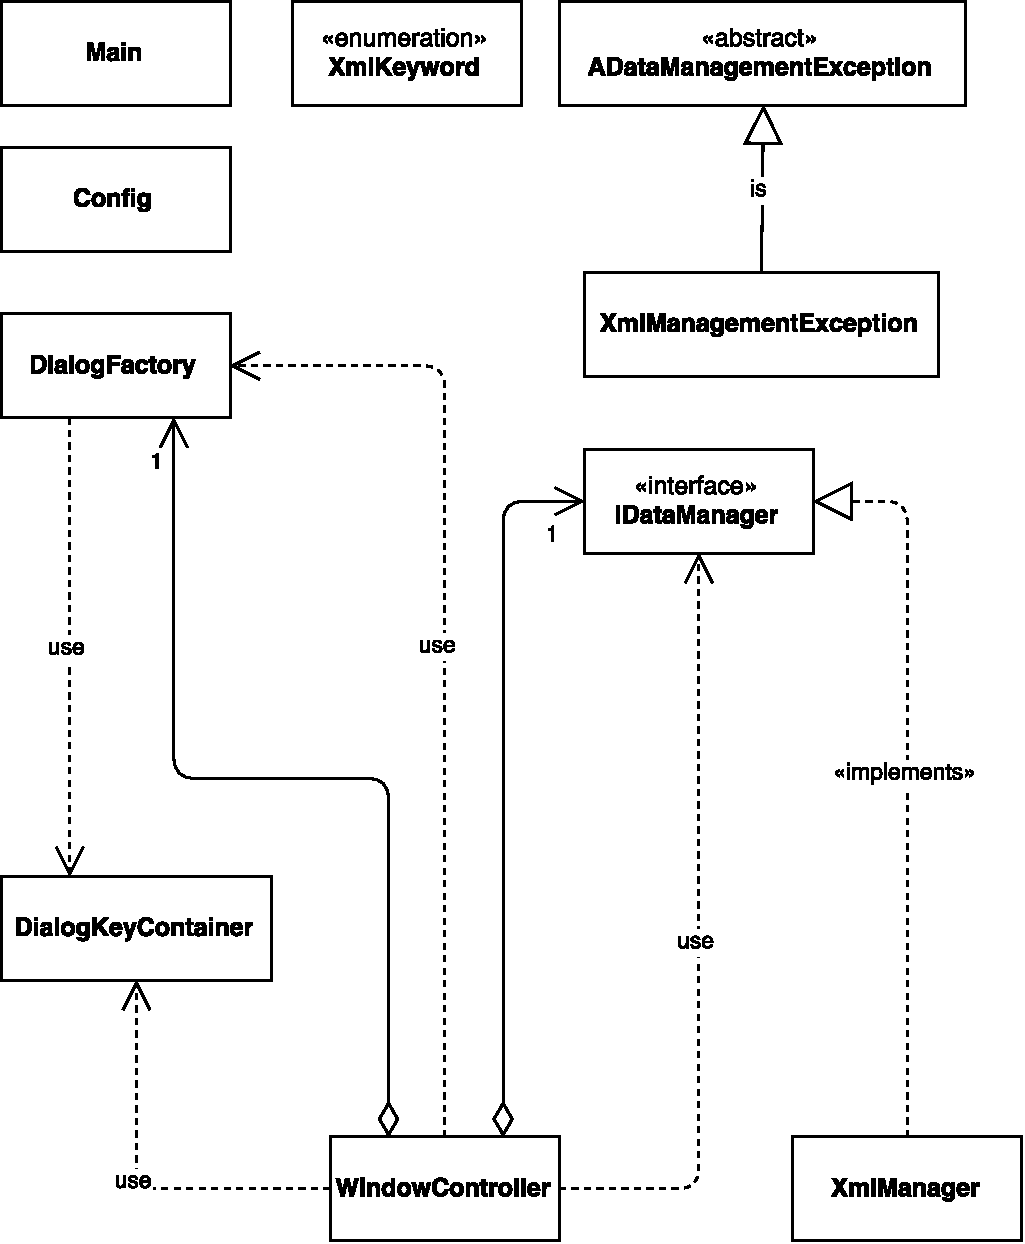
\includegraphics[
    page=1,
    width=\textwidth,
    height=\textheight,
    keepaspectratio
]{uml.pdf}
\end{figure}

\chapter{Uživatelská příručka aplikace}
V~adresáři \texttt{CodeManager/bin} kořenového adresáře vytvořeného programového vybavení, které je součástí této práce, se nachází spustitelný soubor aplikace pro správu zdrojových kódů \texttt{CodeManager.jar}. Po jeho spuštění se otevře hlavní okno uživatelského rozhraní aplikace v~režimu zobrazování zdrojového kódu.\par

\section{Popis uživatelského rozhraní}
V~levé části hlavního okna se nachází seznam uložených tříd v~jazyce Java, pro které byly implementovány knihovny v~ostatních uložených programovacích jazycích, s~tlačítky pro přidání, úpravu nebo odstranění třídy. V~horní části se nachází nalevo (nad seznamem) vyhledávací pole uložených tříd, napravo pak nabídka uložených jazyků, vedle níž se nacházejí tlačítka pro přidání, úpravu nebo odstranění jazyka. Pod nabídkou jazyků (v~pravé části okna) je umístěno textové pole pro zobrazení a úpravu zdrojových kódů a pod ním tlačítka pro kopírování a vkládání kódu a spouštění a ukládání jeho úpravy. V~horní části okna nad vyhledávacím polem a nabídkou jazyků se nachází hlavní menu aplikace, které sdružuje funkcionalitu tlačítek v~okně.

\section{Zobrazení kódu}
Kliknutím na položku v~seznamu tříd v~levé dolní části okna dojde k~jejímu označení. Výběr položky lze provést i zadáním počátečních písmen názvu (nezáleží na jejich velikosti) do textového pole v~levé horní části okna a kliknutím na tlačítko \texttt{Najít}. V~nabídce v~pravé horní části okna lze vybrat programovací jazyk. Jakmile jsou třída i jazyka vybrány, v~textovém poli v~pravé dolní části okna se zobrazí uložený zdrojový kód knihovny představující označenou třídu ve zvoleném jazyce. Dokud se okno nachází v~režimu zobrazení kódu, obsah textového pole je možné pouze prohlížet, označovat jeho části a kopírovat do schránky (pro zkopírování celého obsahu najednou slouží tlačítko \texttt{Kopírovat kód}). Příklad okna aplikace po načtení kódu v~režimu zobrazení ukazuje obrázek \ref{fig:view-code-window}.

\section{Změna v~seznamu tříd}
V~seznamu Java tříd je možné přidávat, upravovat a mazat položky. Přidání položky lze spustit kliknutím na tlačítko \texttt{Přidat třídu}. Zobrazí se dialogové okno, do kterého je nutné zadat název nové třídy. Kliknutím na tlačítko \texttt{OK} v~dialogovém okně se potvrdí přidání nové třídy se zadaným názvem do seznamu uložených tříd a je možné následně uložit zdrojové kódy pro tuto třídu. Pro úpravu označené položky slouží tlačítko \texttt{Upravit třídu}. Následně zobrazené dialogové okno slouží k~zadání nového názvu třídy. Po kliknutí na tlačítko \texttt{OK} se změní název třídy v~seznamu. Uložené zdrojové kódy pro původní název třídy zůstanou zachovány. K~odstranění položky je určeno tlačítko \texttt{Odstranit třídu}. Po kliknutí na toto tlačítko se nejprve zobrazí potvrzovací dialog. Potvrzením pomocí tlačítka \texttt{OK} dojde k~odstranění označené třídy ze seznamu. Uložené zdrojové kódy pro tuto třídu ve všech jazycích budou nenávratně odstraněny.\par
Pro zadávaný název třídy (ať už se jedná o~vytvoření nové třídy nebo změnu názvu existující) platí pravidlo, že musí být validním názvem třídy v~jazyce Java. Může tedy obsahovat pouze číslice (nesmí však číslicí začínat), písmena (velká i malá) a podtržítko. Dále se název nesmí shodovat s~názvem žádné aktuálně uložené třídy, přičemž při porovnávání názvů na shodu se nerozlišuje velikost písmen.

\section{Změna v~seznamu jazyků}
Nabídku programovacích jazyků lze modifikovat stejnými způsoby, jako seznam tříd. Stiskem tlačtka \texttt{Přidat jazyk}, zadáním názvu nového jazyka v~dialogu a potvrzením tlačítkem \texttt{OK} přibude nový jazyk v~nabídce. Data pro každou uloženou třídu je následně možné rozšířit o~zdrojový kód v~tomto nově uloženém jazyce. Stisknutím tlačítka \texttt{Upravit jazyk}, zadáním nového názvu a potvrzením tlačítkem \texttt{OK} se změní název jazyku v~nabídce na nově zadaný. Zdrojové kódy z~předchozího jazyka však zůstanou v~každé třídě zachovány. Po stisku tlačítka \texttt{Odstranit jazyk} a potvrzení tlačítkem \texttt{OK} se odstraní zvolený jazyk z~nabídky uložených jazyků. Uložené zdrojové kódy v~tomto jazyce pro každou třídu budou nenávratně odstraněny.\par
Pravidla pro formát názvu programovacího jazyka jsou méně přísná než v~případě názvů tříd. Název jazyka pouze nesmí začínat a končit mezerou, nesmí obsahovat více po sobě jdoucích mezer a nesmí obsahovat jiné bílé znaky než mezery. Stejně jako pro názvy tříd i zde platí, že se název nesmí shodovat s~názvem aktuálně již uložené položky.

\section{Úprava kódu}
Pokud je vybrána Java třída i programovací jazyk, lze příslušný zdrojový kód upravit pomocí tlačítka \texttt{Upravit kód}. Po stisknutí tlačítka se rozhraní okna přepne do režimu úpravy kódu, jak ukazuje obrázek \ref{fig:edit-code-window}. V~tomto režimu není možné přepnout na jiný jazyk nebo třídu, je však možné editovat zdrojový kód zobrazený do textového pole v~pravé dolní části okna (celý obsah lze poté tlačítkem Vložit změny také najednou nahradit obsahem schránky). Nová podoba kódu se uloží po kliknutí na tlačítko \texttt{Uložit změny}. Provedené změny v~kódu je možné zahodit stisknutím tlačítka \texttt{Zrušit úpravy} a potvrzením zrušení pomocí tlačítka \texttt{OK} v~dialogovém okně (stejný potvrzovací dialog se v~tomto režimu zobrazí i při pokusu o~ukončení aplikace). V~takovém případě se načte zpět původní podoba kódu a provedené změny jsou ztraceny. Bezprostředně po uložení nebo zrušení změn se rozhraní okna přepne zpátky do režimu prohlížení kódu, kde je možné přepínat položky v~seznamu tříd nebo v~nabídce jazyků.

\begin{figure}
\caption{Okno aplikace -- režim zobrazení kódu}
    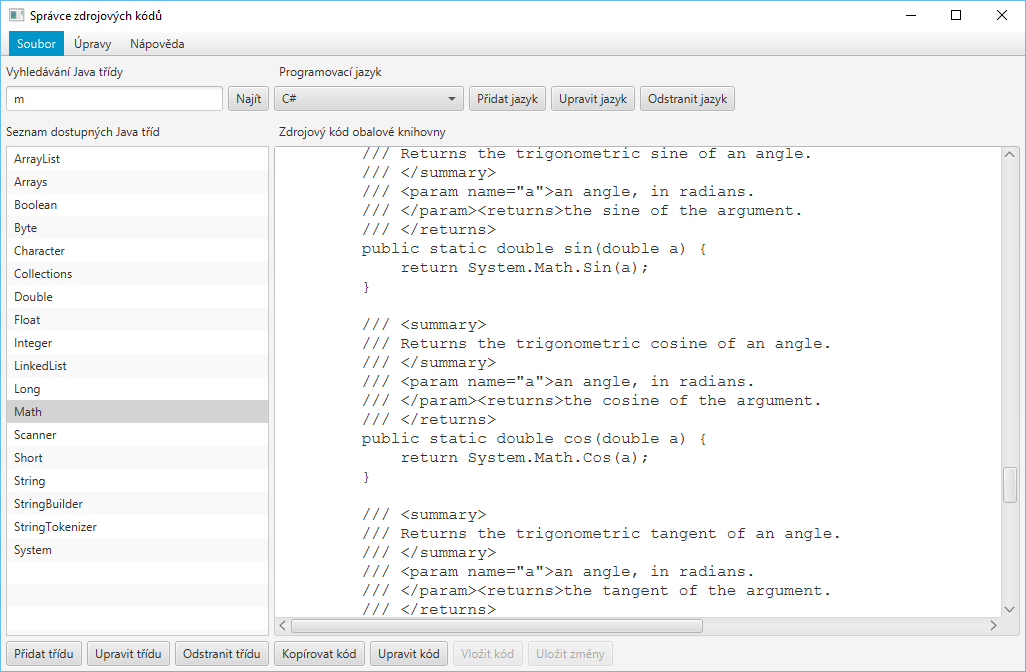
\includegraphics[
    width=\textwidth,
    height=\textheight,
    keepaspectratio
]{view-code.png}
\label{fig:view-code-window}
\end{figure}

\begin{figure}
\caption{Okno aplikace -- režim úpravy kódu}
    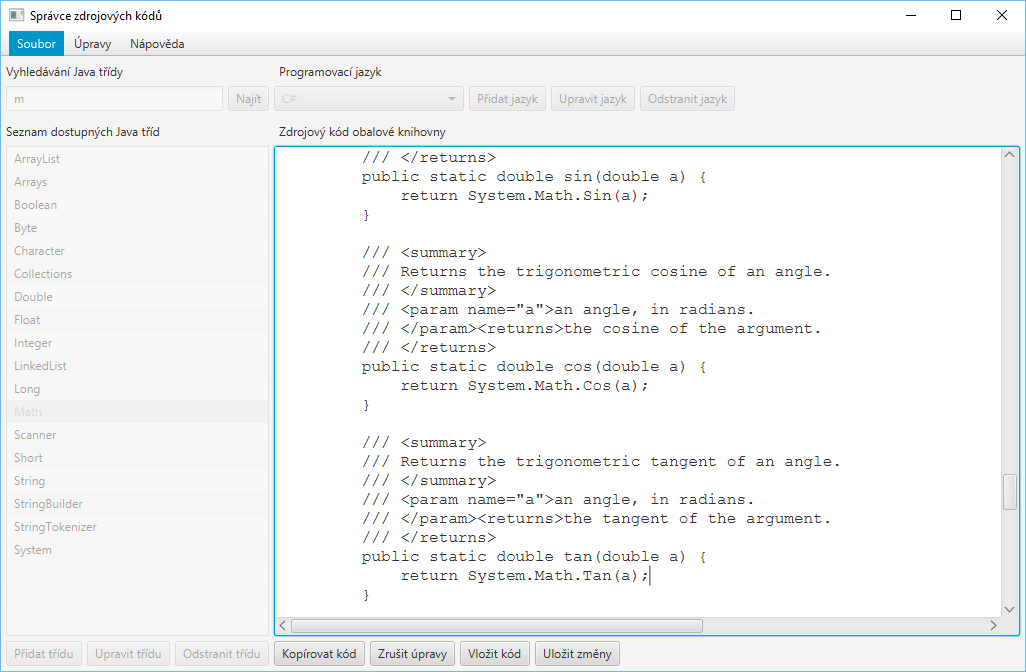
\includegraphics[
    width=\textwidth,
    height=\textheight,
    keepaspectratio
]{edit-code.png}
\label{fig:edit-code-window}
\end{figure}

\chapter{Nástroj pro převod kódu}
K~usnadnění převodu kódu psaném v~jazyce Java do jiných jazyků byl vytvořen jednoduchý nástroj s~webovým rozhraním. Soubor \texttt{index.html} pro jeho otevření v~okně webového prohlížeče se nachází v~adresáři pojmenovaném \texttt{CodeConverter}, nacházejícím se v~kořenovém adresáři vytvořeného programového vybavení. Ukázka webového rozhraní nástroje je na obrázku \ref{fig:convert-helper-page}

\section{Popis uživatelského rozhraní}
V~horní části webového rozhraní pod popisem nástroje se nachází přepínače pro nastavení programovacího jazyka, do kterého bude kód převáděn. Pod nimi se nachází dvě textová pole. Pole v~levé části je editovatelné a je určeno k~zadání původního zdrojového kódu jazyka Java. Pole v~pravé části slouží k~zobrazení výsledku a je určeno pouze pro čtení.

\section{Převod kódu}
Vkládáním kódu do vstupního textového pole je automaticky spouštěn převod a jeho výsledky jsou vypisovány do výstupního textového pole. Nástroj pro správnou funkci vyžaduje v~prohlížeči spuštěnou podporu jazyka JavaScript, ve kterém je psán převodní skript. Nástroj neprovádí komplexní převod a neprodukuje konečnou podobu kódu, poskytuje však možnost automatizace jednoduchých úkonů, jako je například přepis pojmenování datových typů a některých dalších klíčových slov.

\section{Konfigurace}
Skript pro převod kódu se nachází ve složce scripts v~adresáři nástroje. Pro převody kódu používá soustavu regulárních výrazů sdružených s~výslednými řetězci v~jednoduchých objektech (atribut \texttt{p} obsahuje regulární výraz představující vzor nahrazovaných řetězců, atribut \texttt{r} obsahuje řetězec, kterým jsou výskyty vzoru nahrazovány), které jsou ukládány do polí pro každý programovací jazyk zvlášť. Funkcionalitu skriptu je možné jednoduše rozšířit přidáním dalších objektů s~regulárními výrazy do příslušných polí, která jsou umístěna na začátek skriptu.

\begin{figure}
\caption{Nástroj automatického převodu kódu}
    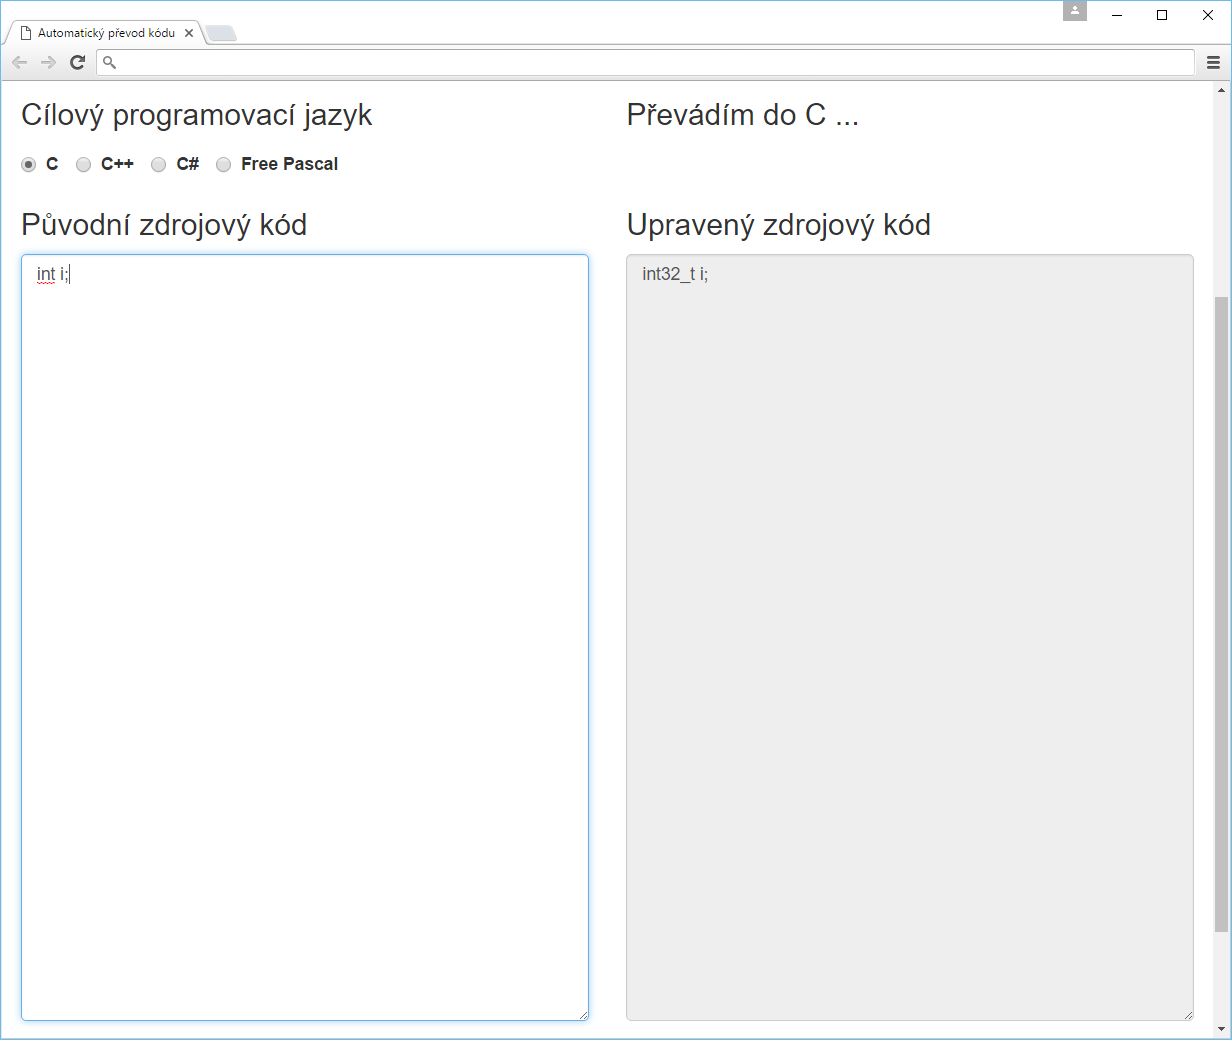
\includegraphics[
    width=\textwidth,
    height=\textheight,
    keepaspectratio
]{convert-helper.png}
\label{fig:convert-helper-page}
\end{figure}

\end{document}
